\documentclass[main]{subfiles}

\begin{document}
% Chapter Template
\setcounter{chapter}{3}

% Results
%  Creatures with uncoupled sinusoidal oscillators
%  Simple limiter control in the simulator
%   Indirect limiter control through the morphology
%   Direct limiter control through the sensor feedback
%    Limiting the Model Leg in the Minemonics simulator
%    Evolved examples 
\chapter{Results} % Main chapter title

\label{Chapter\thechapter} % Change X to a consecutive number; for referencing this chapter elsewhere, use \ref{ChapterX}

\lhead{Chapter \thechapter. \emph{Results}} % Change X to a consecutive number; this is for the header on each page - perhaps a shortened title

\section{Creatures with uncoupled sinusoidal oscillators}

In the first experimental setting, the sinusoidal controller as described in \ref{sec:sinusoidal-oscillators} was used to evolve creatures. A population of 100 creatures was set up with an average velocity fitness function and a minimal height fitness function. The latter was chosen because the simulator had issues in the physical model setup that led to creatures that could fly due to imaginary forces (as described in \ref{subsec:population}). The minimal height fitness function punished those creatures that reached a high average height of all limbs, which was the case for creatures that were flying. The simulation was run for approximately a day and took 181 generations for locomotion behavior to occur. Every creature was evaluated for 20 seconds. 181 generations of 100 creatures evaluated for 20 seconds are \(\approx\unit[4.2]{days}\), however, since the simulator can evaluate faster than real-time if the simulation permits it, it could simulate the creatures with approximately \(4.2\) times real-time. The successful solutions evolved can be seen below in figure \ref{figure:successfulcreatures}.

\begin{figure}[H]
\centering
\missingfigure[figwidth=1\textwidth]{Figure of the successful sinusoid controller creatures.}
\caption[Figure of the successful sinusoid controller creatures.]{Figure of the successful sinusoid controller creatures.}
\label{figure:successfulcreatures}
\end{figure}

Creatures that exhibit successful locomotion seem to share a common ancestor that was the first who evolved a successful walking pattern, since all of them share a similar magenta skin coloring. Since the skin color is randomly set for one limb, the common ancestor could only have had all the same color and must have been replicated using crossover. In crossover (as described in \ref{subsec:crossover}), subsections of the two participating creature genotypes are taken and combined into one new genotype. Since this process involves no mutations, the crossover must have happened mainly among creatures sharing the same magenta skin coloring. Due to the elitism mechanism of the evolutionary process, the first successful creature generated an onset of an avalanche of successful creatures flooding the population with very similar solutions. 

However, the major drawback of the sinusoidal oscillator controller is that they do not show any adaption during the evaluation depending on the environment. The only way for the controller to adapt is on the evolutionary time-scale through mutation, which does not result in an advantage for the individual in its evaluation, but only helps a future generation of the individual to eventually converge to a new, applicable solution.
\todo[inline]{Show reason why the creatures can not adapt.}
\section{Simple limiter control in the simulator}
% rev. 2

The second type of controller is a reaction to the fixed oscillatory motion scheme of the sinusoidal controller, which in reality is highly improbable to be existing in a natural animal. Furthermore it could fix the inability to adapt to environmental disturbances. The controller using an underlying chaotic system could be a marvellous source of periodic patterns of motion due to its infinite number of unstable periodic orbits. If a creature could use simple limiter control to stabilize UPOs and exploit the periodic orbits for locomotion patterns, this could lead to a more robust and adaptive way of motion. Experimentally, this would mean that if the creatures exhibit periodic locomotion patterns that it could be shown that the successful creatures controlled the amount of chaotic movement of the controller or the chaotic movement of the limb and stabilized unstable periodic orbits to exploit it for limb motion. Showing that the controller or limb motion is less chaotic can be shown by calculating the largest Lyapunov exponent, which accounts for the amount of divergence of two slightly different initial conditions of the controller or the limb motion.

The experiments were run on the chaotic controller as described in \ref{subsec:chua-circuit}. Simple limiters can come in various ways, since they only must be natural to the system at hand \cite{bib:Corron2000}. Therefore the first experiments were run using chaotic controllers without direct limiters implemented to the controllers. Unfortunately, this approach was not successful as no periodic limb motion could be observed at any time of the evolution, meaning that the morphology can not act as a limiter to control the chaos at any point if the chaotic system does not get any feedback from the morphology. The second idea was to implement limiters based on the sensory feedback of the respective joint the controller is controlling.

\subsection{Indirect limiter control through the morphology}
% rev. 1

The first experiments were run using chaotic controllers without direct limiters. The controllers start with different initial conditions and different integration speeds, but are not limited using sensory input. Therefore the chaotic trajectories emitted from the controllers are only limited through the morphology. The experiment conducted was run using 4 different settings in terms of evaluation time and number of creatures in the population. However, the desired limiter control exhibiting periodic or quasi-periodic motion could not be observed in any of the creatures. This could be explained due to the lacking feedback from the limb to the chaotic system itself. Therefore the chaotic system runs completely uninfluenced and is independent of the limb being limited in its movement. Therefore the next experiment takes the sensor feedback into account to perform implicit limiter control as described in the next section.

\subsection{Direct limiter control through sensory feedback}
% rev. 1

For the second experiment uses a locally influenced chaotic controller. The chaotic controller output is ruled by the three differential equations defining \(\frac{dx}{dt},\frac{dy}{dt} \text{ and } \frac{dz}{dt}\) of which, after integration, it holds the current state of the system in \(x(t),y(t) \text{ and } z(t)\).  In this experiment, the controller is limited using the position sensor and the velocity sensor of the joint degree of freedom the controller controls. The controller state \(x(t)\) is replaced by the position sensor output and the controller state \(y(t)\) is replaced by the velocity sensor output. This limiter setup is chosen arbitrarily to observe the influence on a chaotic system. The limiter system imposes limiters on two of the three dimensions in the situation where the limb motion itself is limited due to collision with ground or other limbs, then the joint velocity of the DoF drops and the position comes to a halt. This limits the chaotic controller in two different ways, and it is in question what trajectories will be generated by the system. If it is found to be experimentally successful and the trajectories exhibit periodic or quasi-periodic movement or interleaving periodic-chaotic sequences different from the usual intrinsic chaotic motion of the underlying chaotic system, it will be used in evolutionary settings to evolve creatures controlled with it.

\subsubsection{Limiting the model leg in the simulator}

To test the approach on a simple model organism, we first test the different limiter configurations that use the z(t) as an output.

\begin{figure}[H]
	\centering
	\begin{subfigure}[c]{0.45\textwidth}
	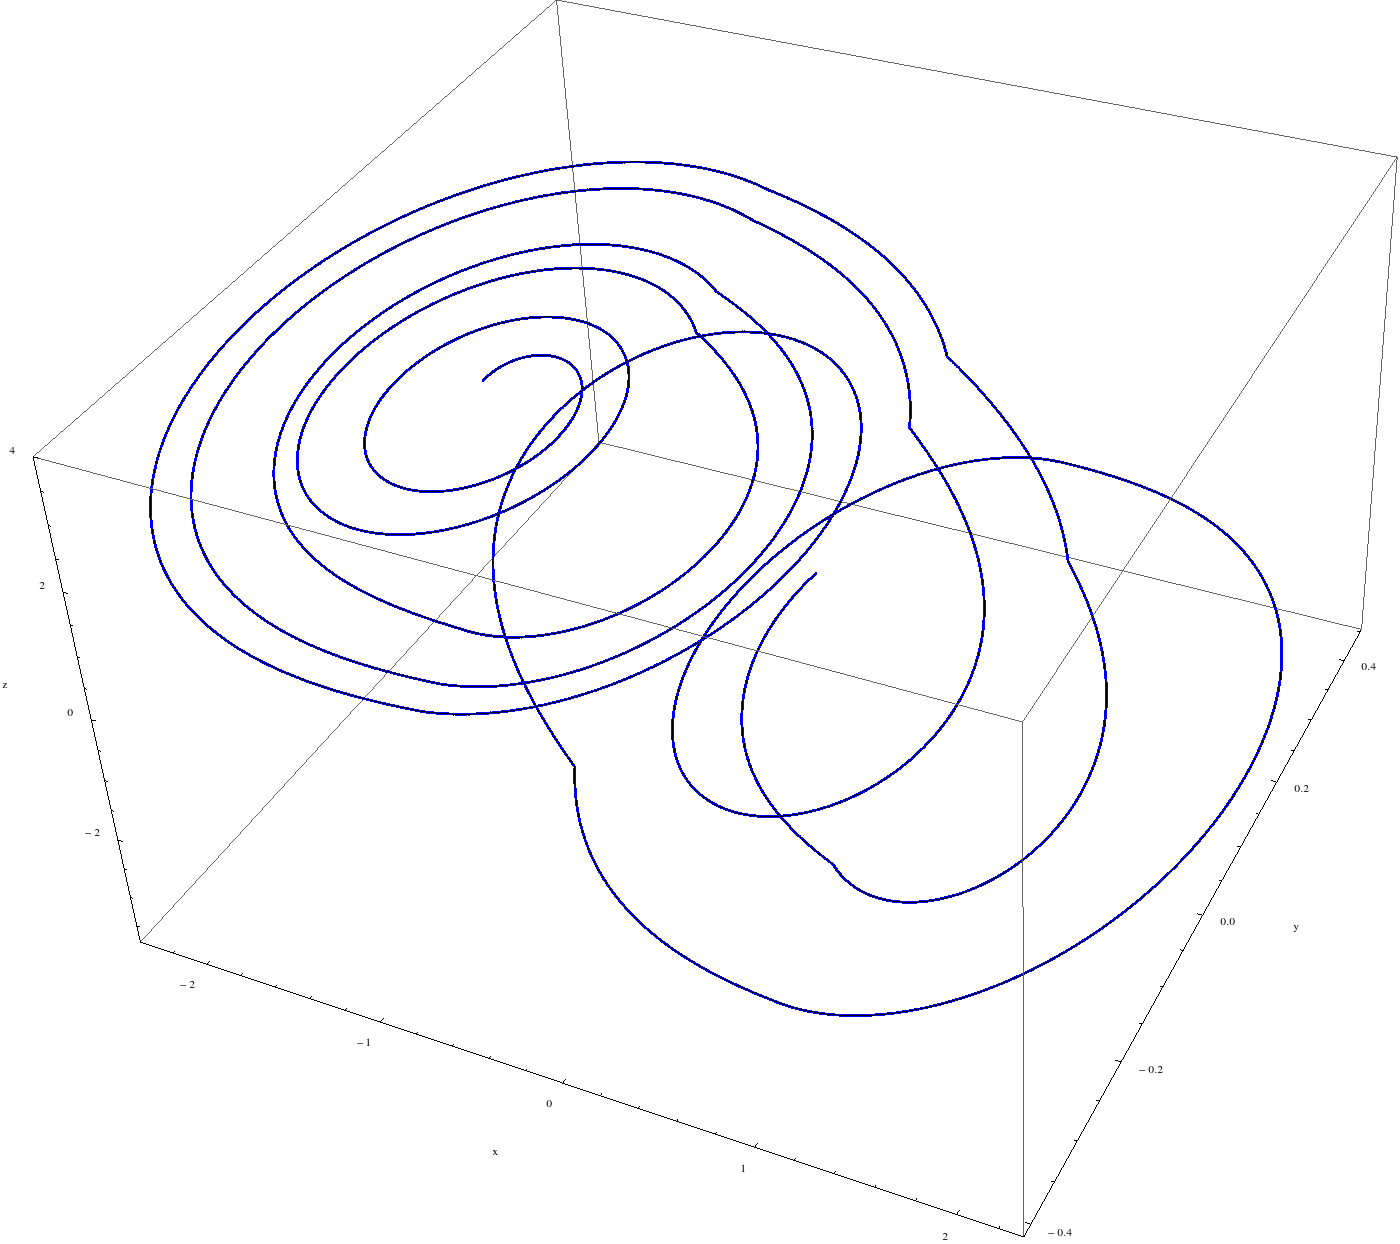
\includegraphics[width=\textwidth]{model-organisms/model-leg/Modelleg-0g-100s-friction00-force0-7-damping0-05-(x)(-1-5)(y)z.png}
	\end{subfigure}
	\begin{subfigure}[c]{0.45\textwidth}
	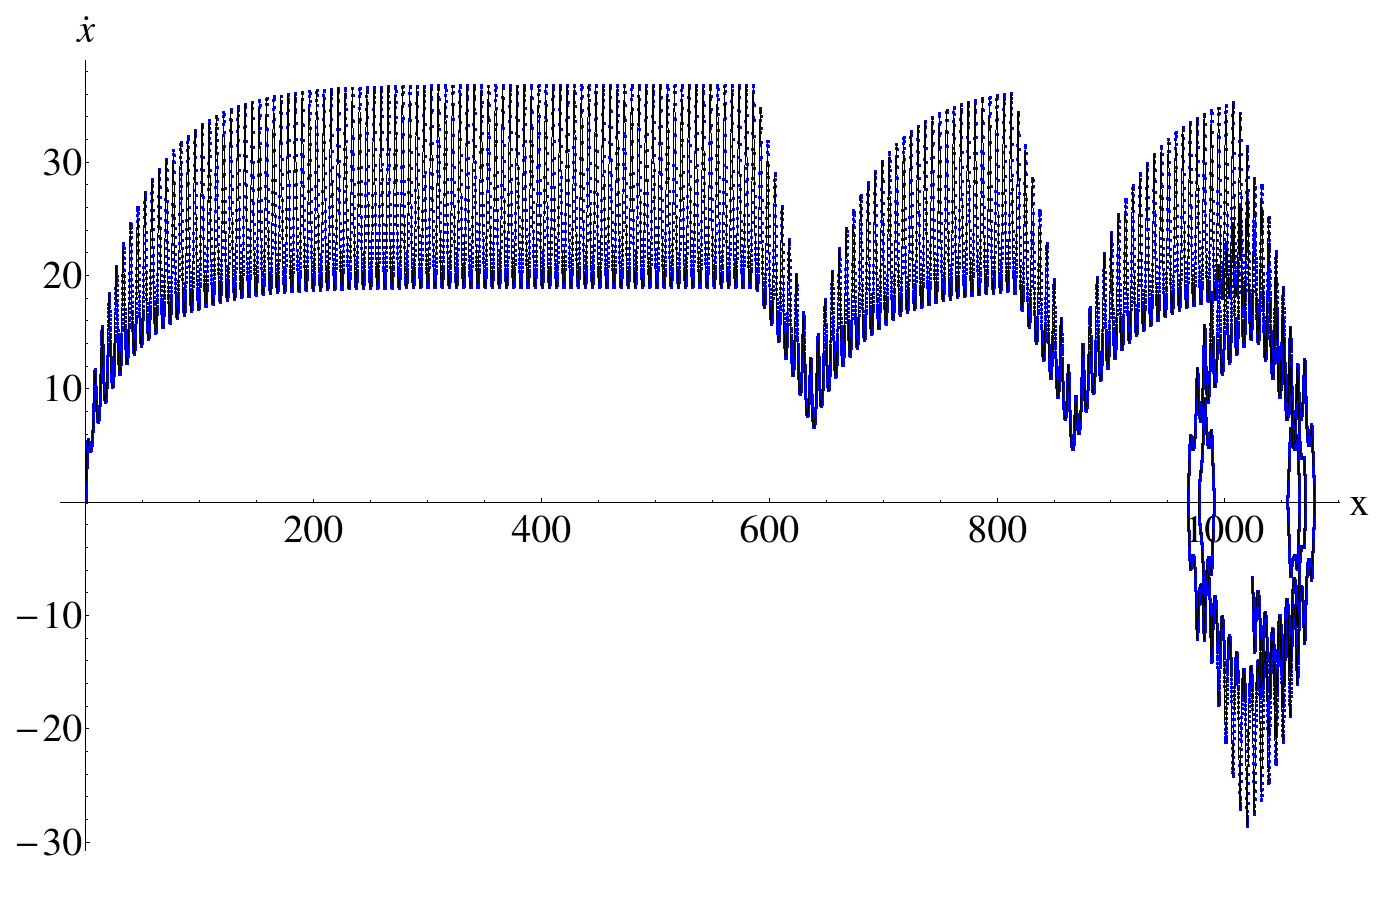
\includegraphics[width=\textwidth]{model-organisms/model-leg/Modelleg-0g-100s-friction00-force0-7-damping0-05-(x)(-1-5)(y)z-joint.png}
	\end{subfigure}
	\caption[Figure of chaotic behaviors in range 2.4-3.19]{Gravity: 0g, Sensors: None, Output: z(t) \(\rightarrow\) Joint torque, Friction: Creature 0, Ground 0, Torque scaling curve:\(0.7~(mass_1~\cdot~mass_2)\)}

	\label{figure:z-2.4-3.19-chaotictrajectories}
\end{figure}

\begin{figure}[H]
	\centering
		\begin{subfigure}[c]{0.45\textwidth}
	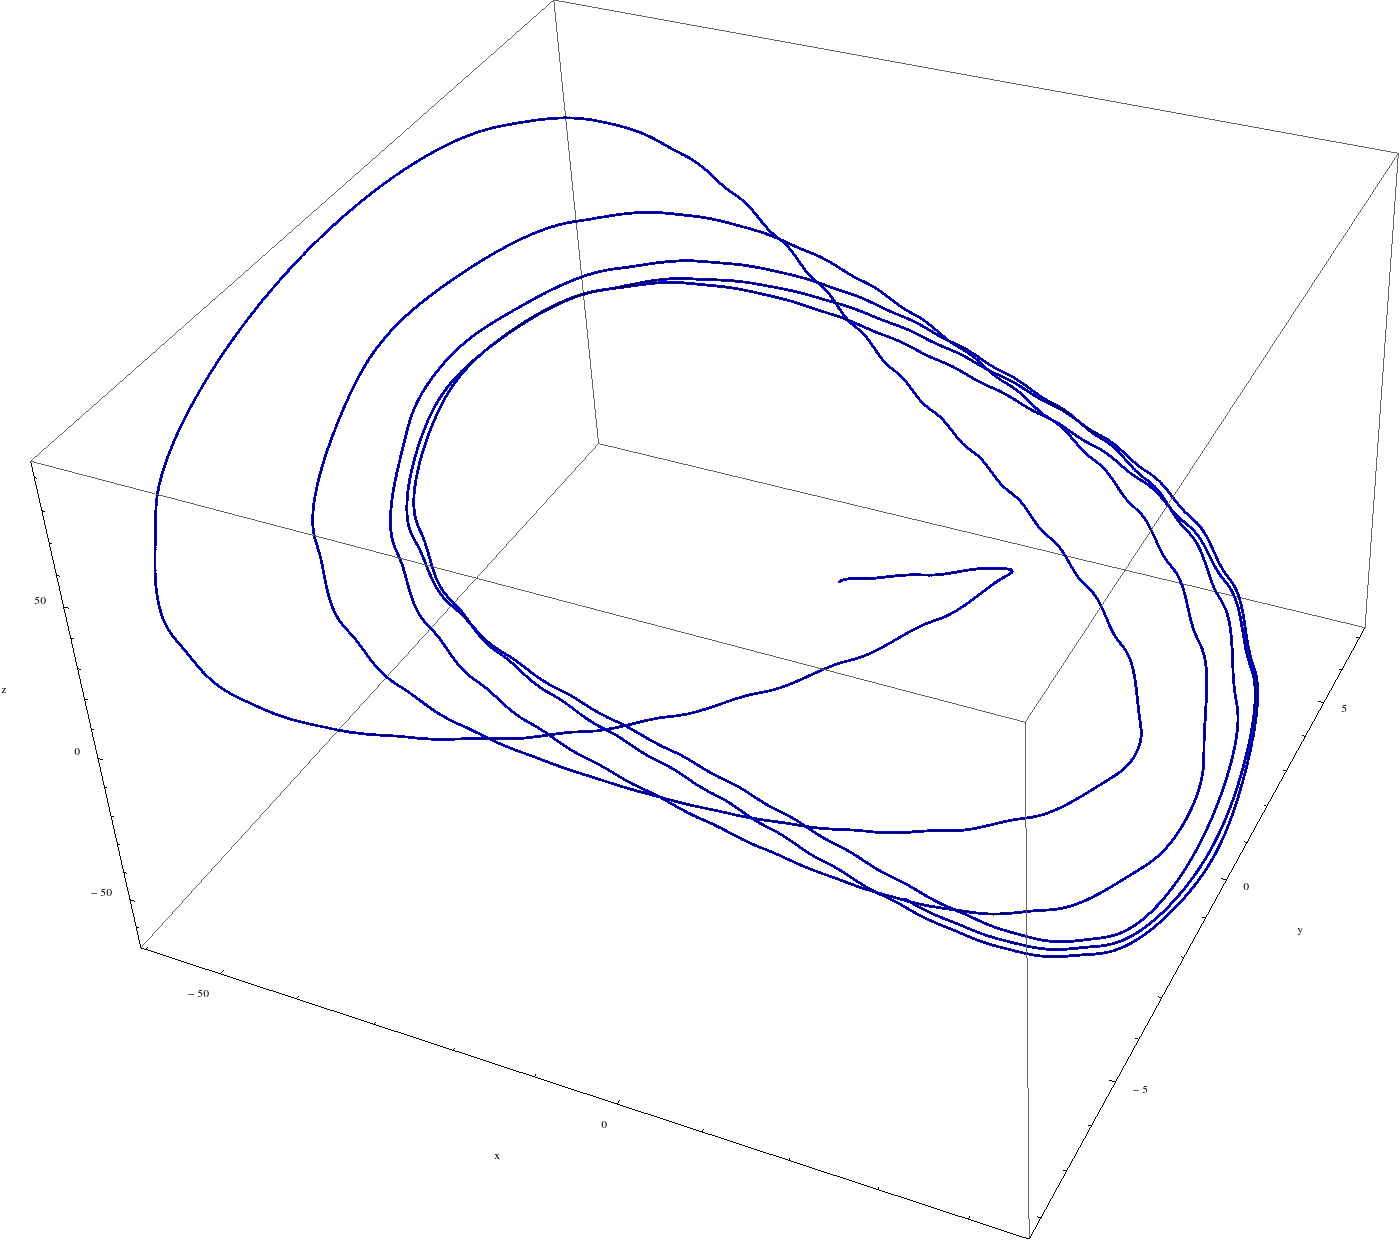
\includegraphics[width=\textwidth]{model-organisms/model-leg/Modelleg-px(y)z-0g-force-0-00007-damping-0.png}
		\end{subfigure}
	\begin{subfigure}[c]{0.45\textwidth}
	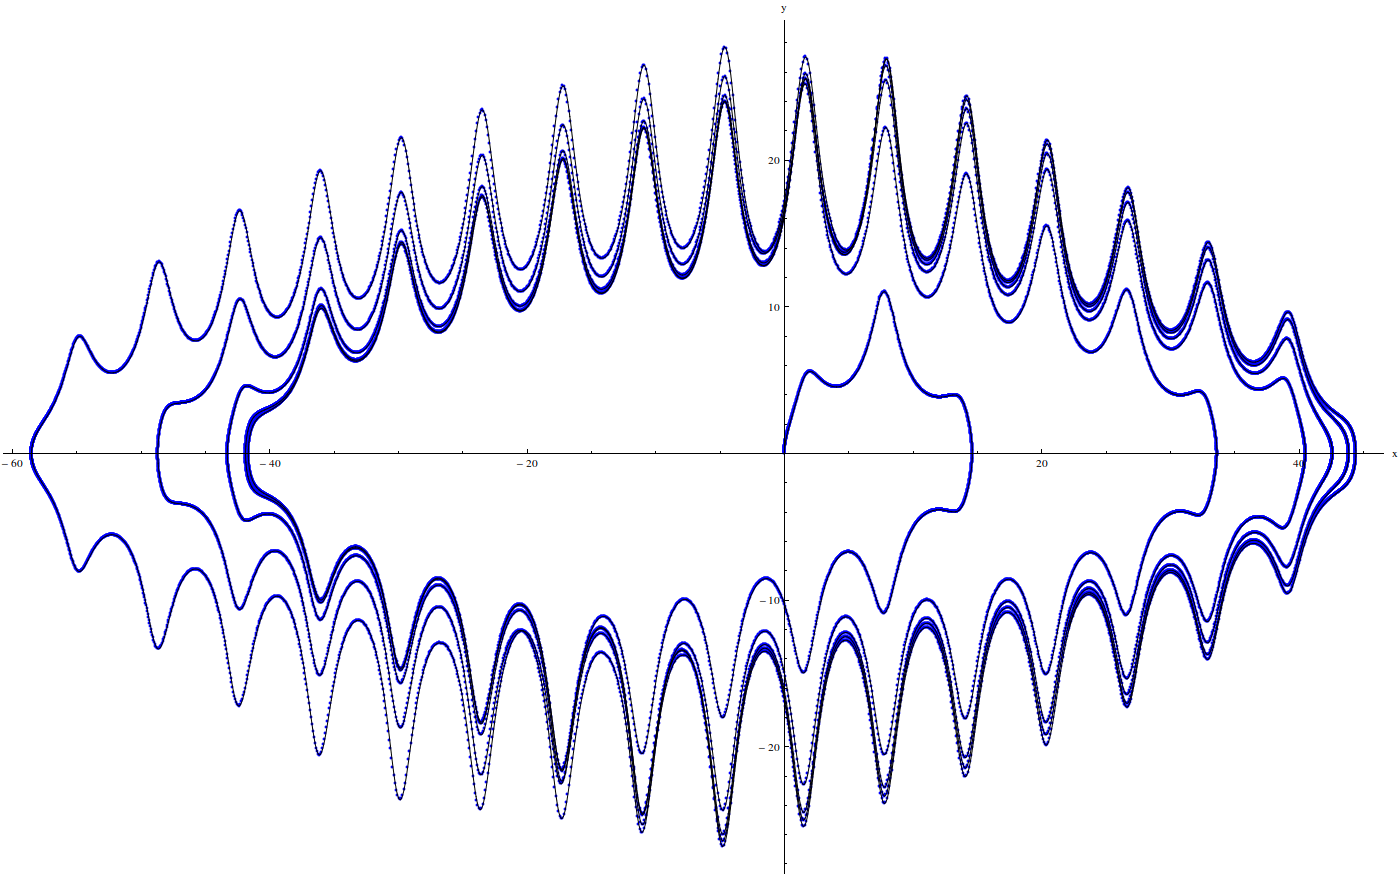
\includegraphics[width=\textwidth]{model-organisms/model-leg/Modelleg-px(y)z-0g-force-0-00007-damping-0-joint.png}
		\end{subfigure}
	\caption[Figure of chaotic behaviors in range 2.4-3.19]{Gravity: 0g, Sensors:  Joint position \(\rightarrow\) x(t),Joint Velocity \(\rightarrow\) y(t), Output: z(t) \(\rightarrow\) Joint torque, Friction: Creature 0, Ground 0, Torque scaling curve:\(0.7~(mass_1~\cdot~mass_2)\)}

	\label{figure:z-2.4-3.19-chaotictrajectories}
\end{figure}

\begin{figure}[H]
	\centering
		\begin{subfigure}[c]{0.45\textwidth}
	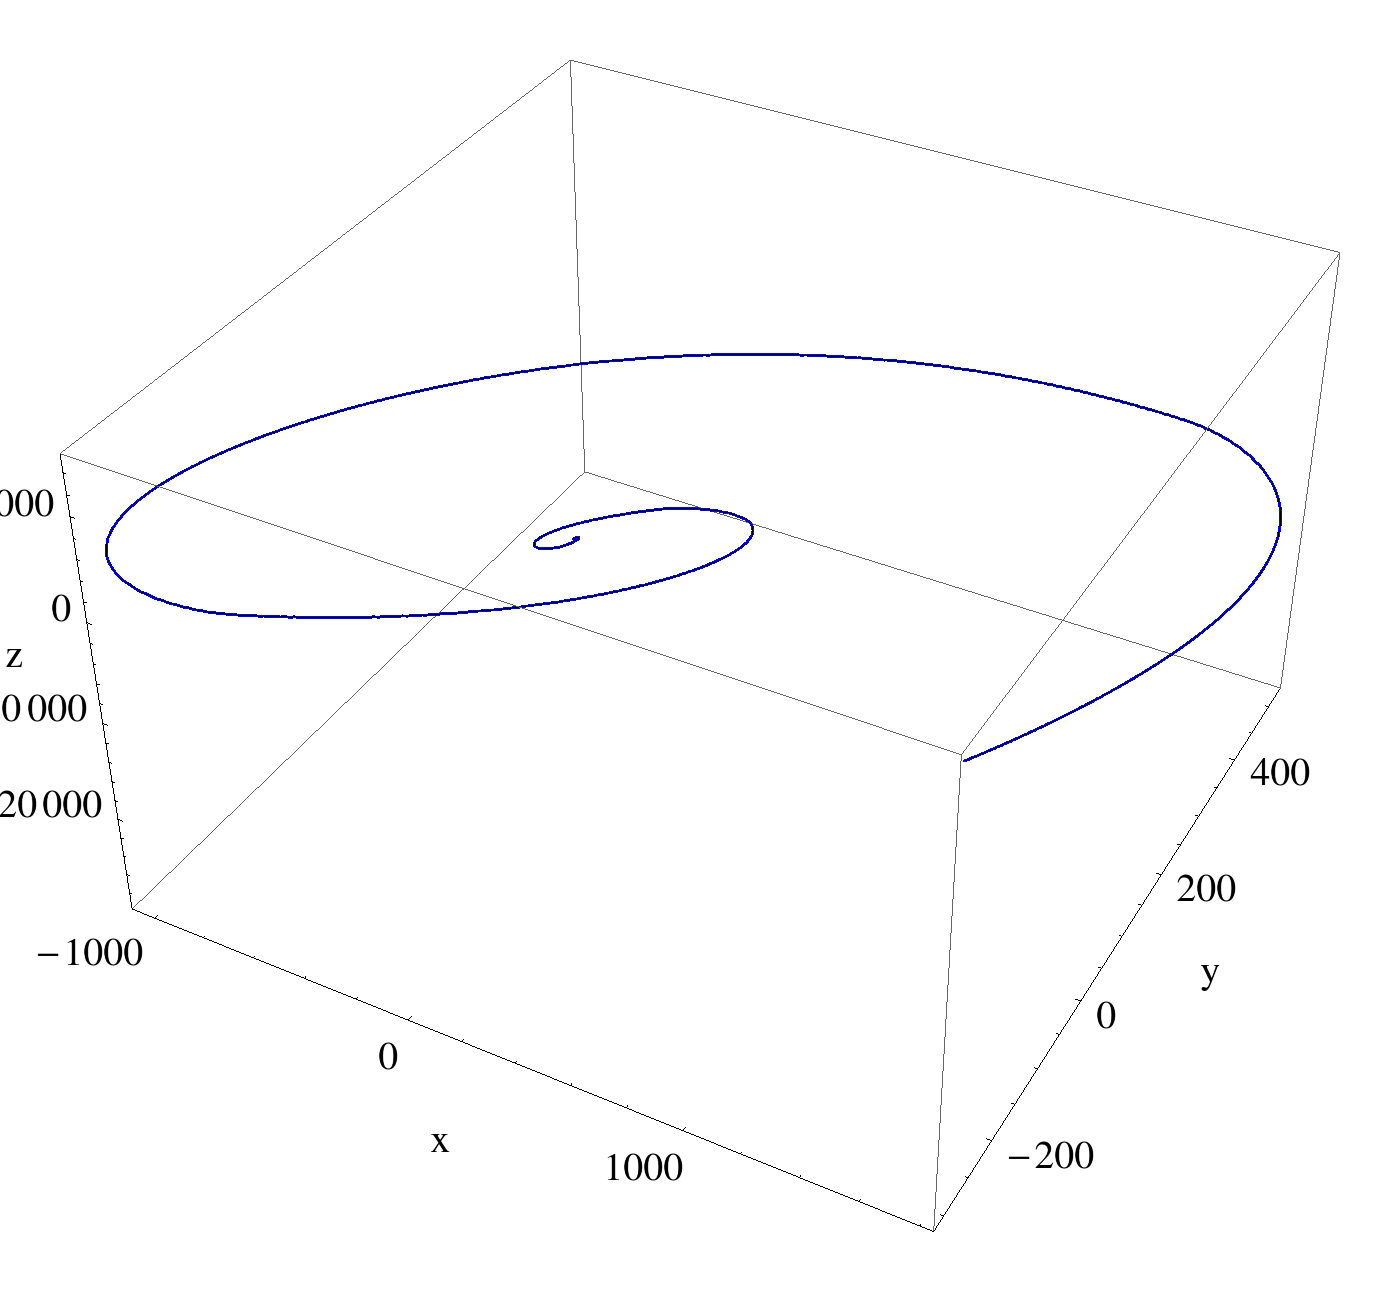
\includegraphics[width=\textwidth]{model-organisms/model-leg/Modelleg-(x)pyz-0g-force-0-00007-damping-0.png}
		\end{subfigure}
	\begin{subfigure}[c]{0.45\textwidth}
	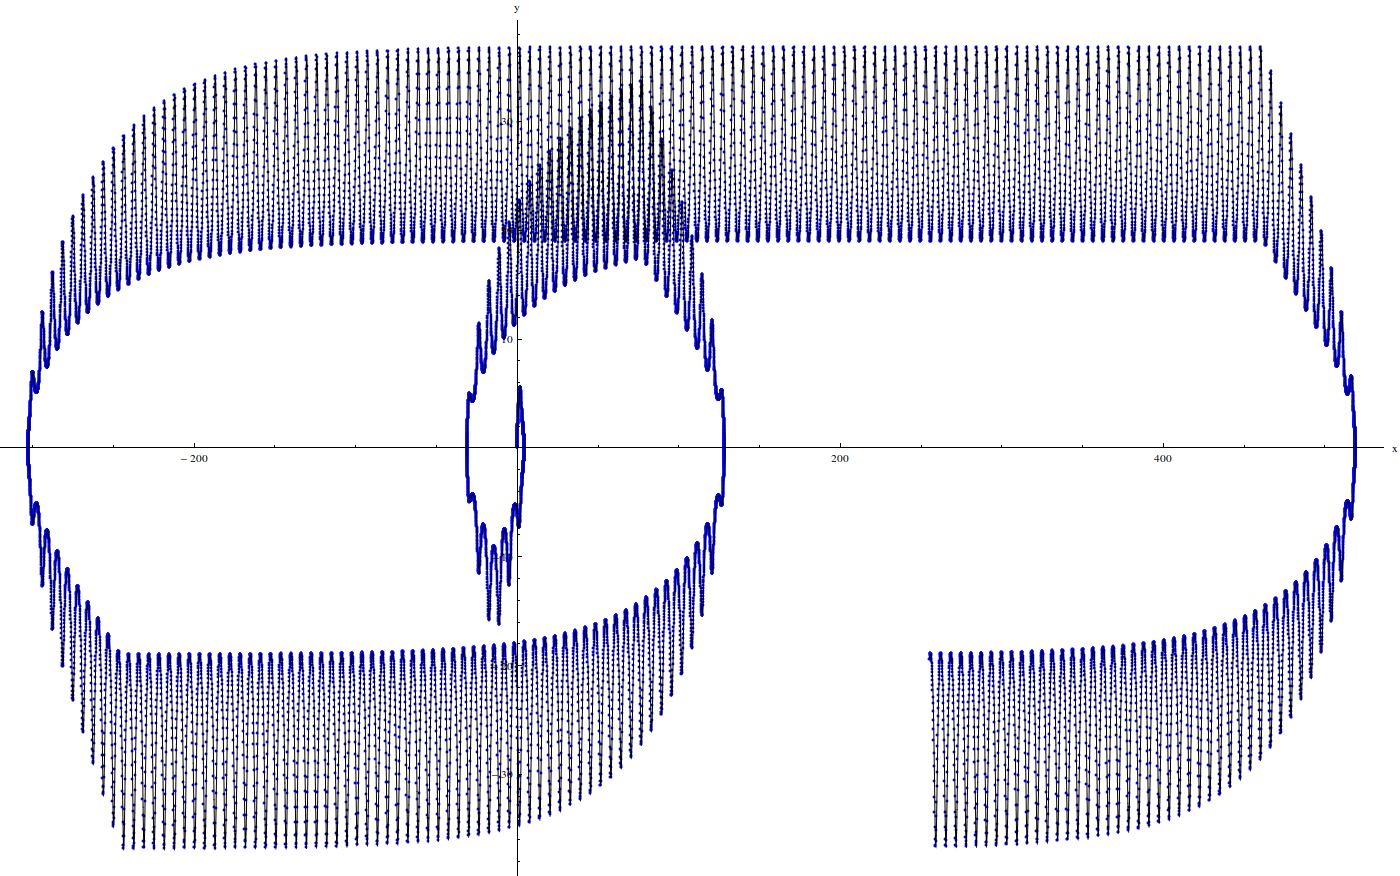
\includegraphics[width=\textwidth]{model-organisms/model-leg/Modelleg-(x)pyz-0g-force-0-00007-damping-0-joint.png}
		\end{subfigure}
	\caption[Figure of chaotic behaviors in range 2.4-3.19]{Gravity: 0g, Sensors:  Joint position \(\rightarrow\) x(t),Joint Velocity \(\rightarrow\) y(t), Output: z(t) \(\rightarrow\) Joint torque, Friction: Creature 0, Ground 0, Torque scaling curve:\(0.7~(mass_1~\cdot~mass_2)\)}

	\label{figure:z-2.4-3.19-chaotictrajectories}
\end{figure}

\begin{figure}[H]
	\centering
		\begin{subfigure}[c]{0.45\textwidth}
	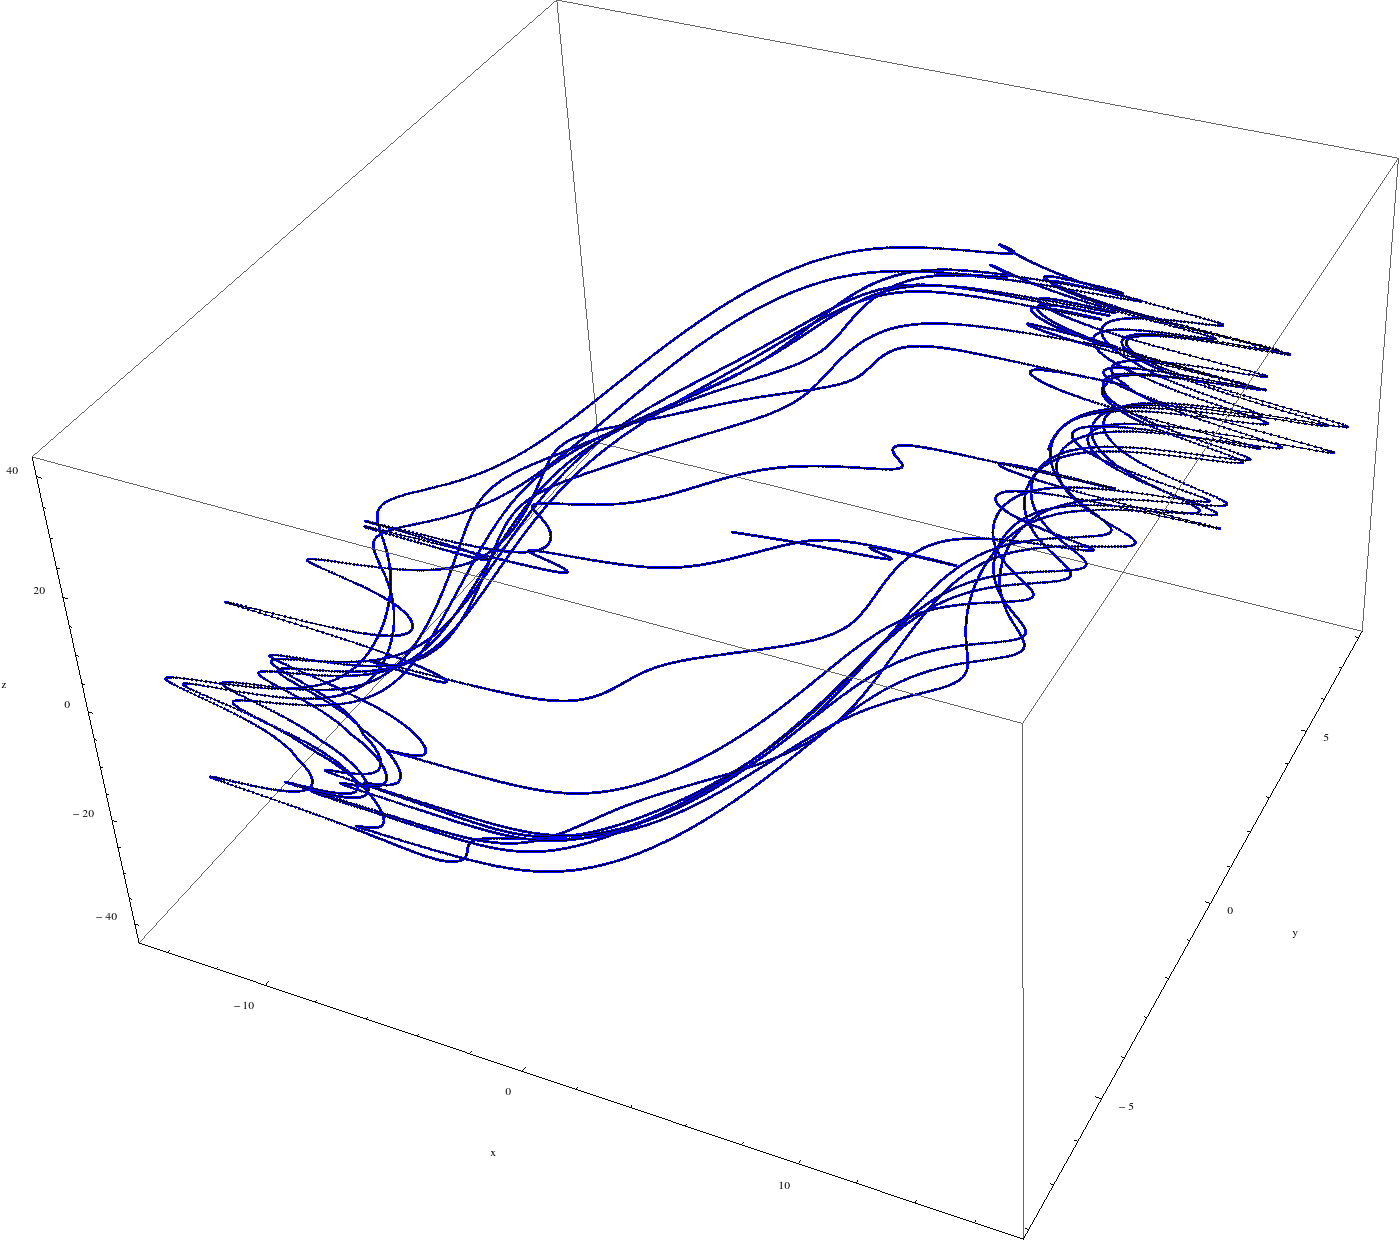
\includegraphics[width=\textwidth]{model-organisms/model-leg/Modelleg-vx(y)z-0g-force-0-00007-damping-0.png}
		\end{subfigure}
	\begin{subfigure}[c]{0.45\textwidth}
	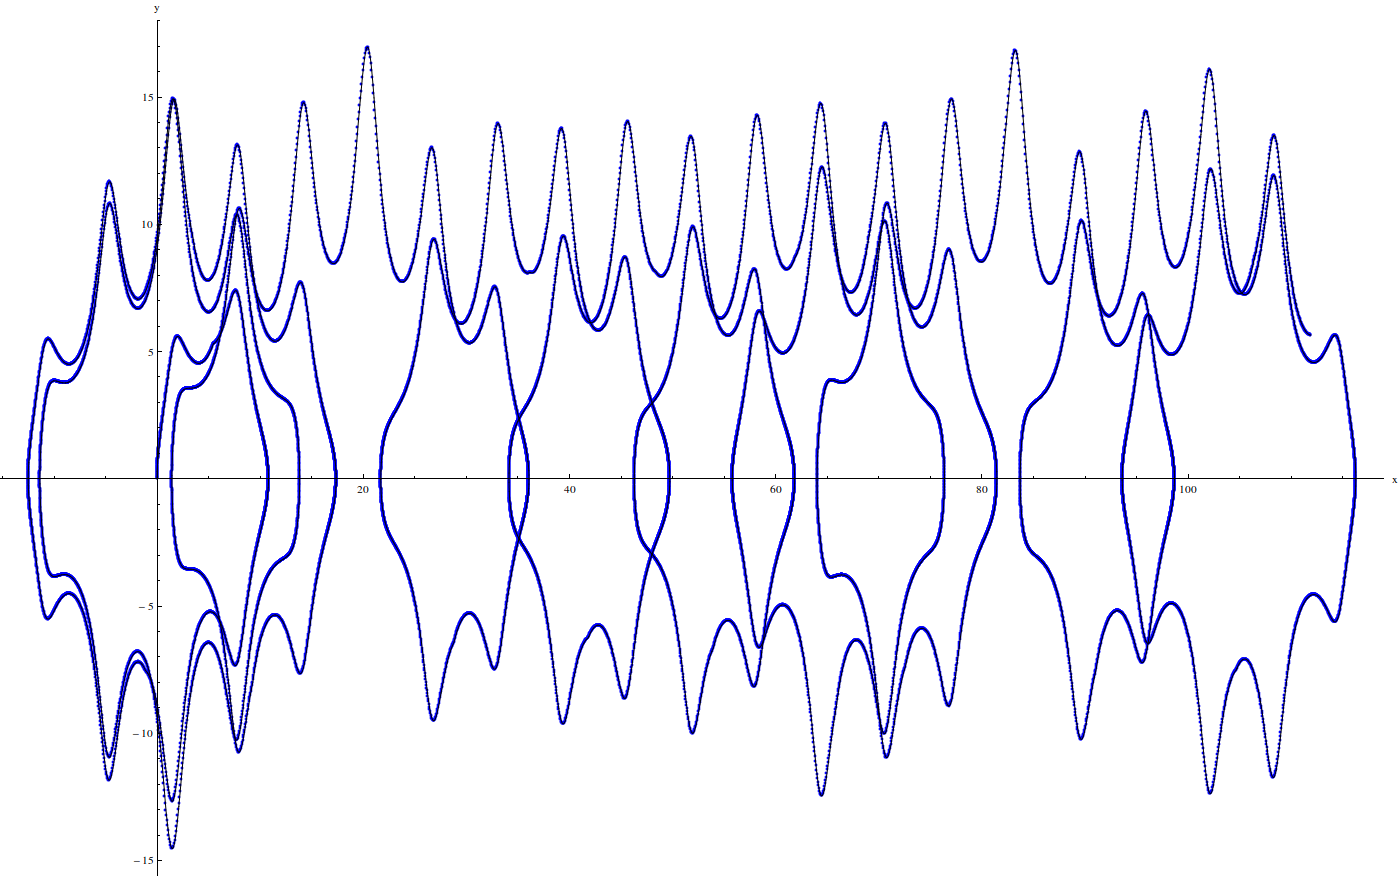
\includegraphics[width=\textwidth]{model-organisms/model-leg/Modelleg-vx(y)z-0g-force-0-00007-damping-0-joint.png}
		\end{subfigure}
	\caption[Figure of chaotic behaviors in range 2.4-3.19]{Gravity: 0g, Sensors:  Joint position \(\rightarrow\) x(t),Joint Velocity \(\rightarrow\) y(t), Output: z(t) \(\rightarrow\) Joint torque, Friction: Creature 0, Ground 0, Torque scaling curve:\(0.7~(mass_1~\cdot~mass_2)\)}

	\label{figure:z-2.4-3.19-chaotictrajectories}
\end{figure}

\begin{figure}[H]
	\centering
		\begin{subfigure}[c]{0.45\textwidth}
	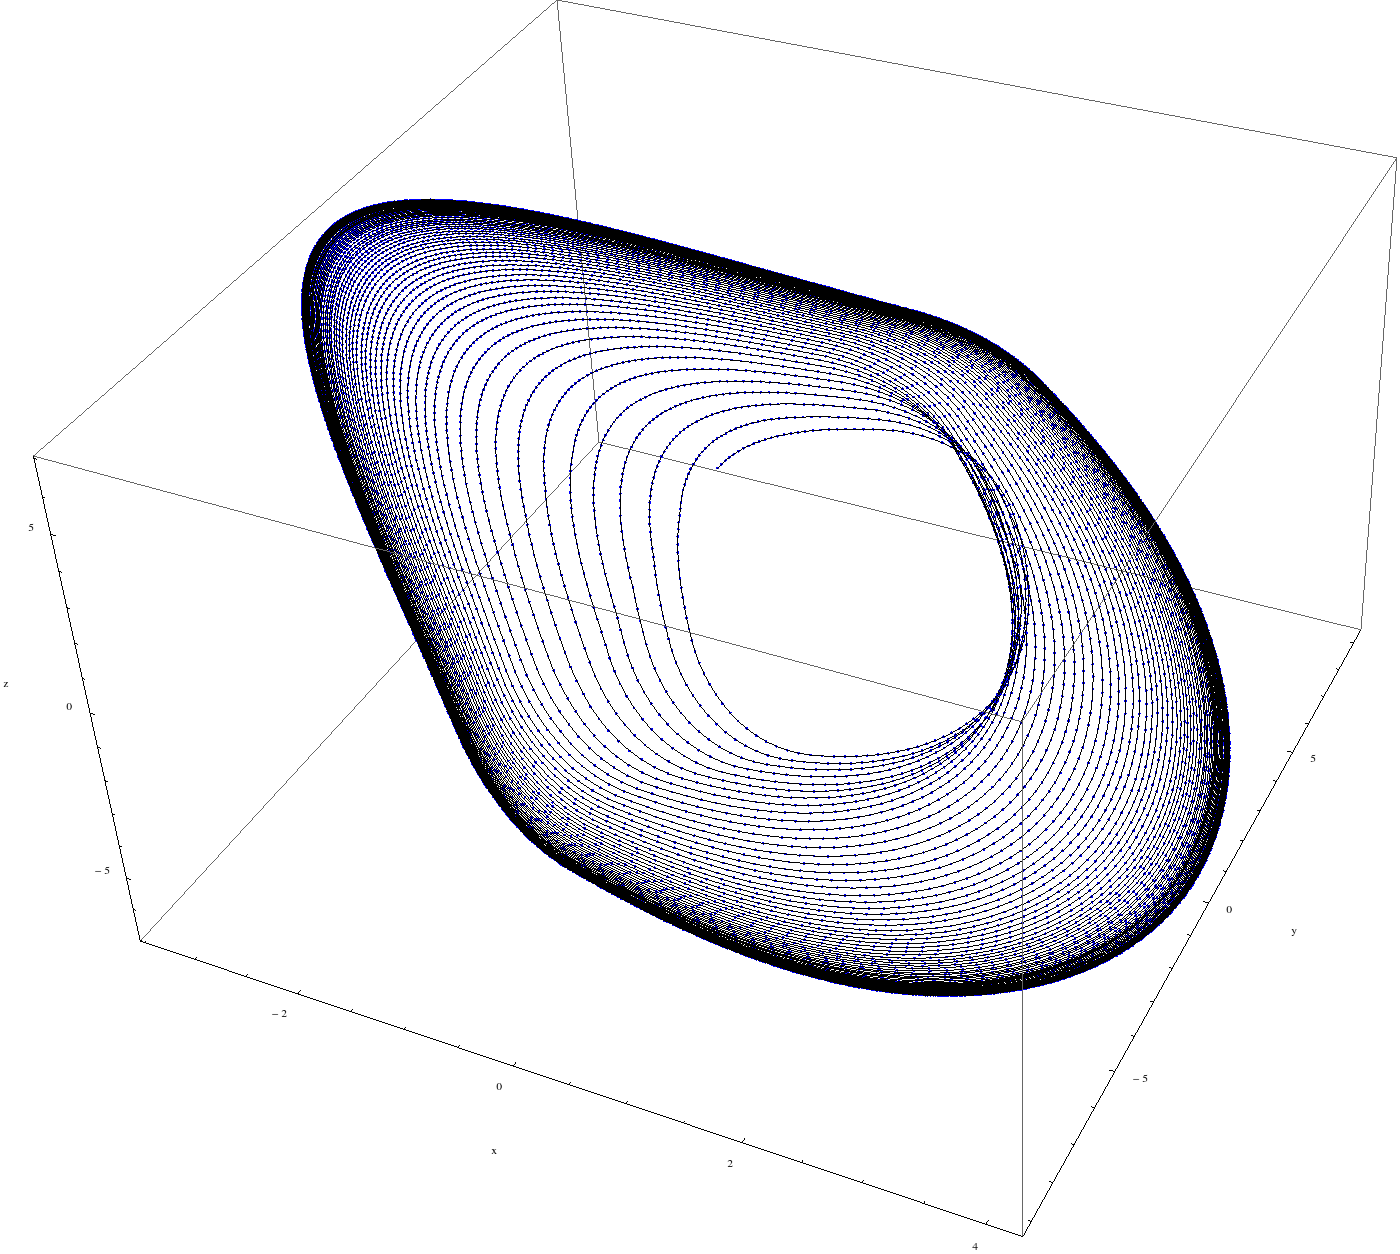
\includegraphics[width=\textwidth]{model-organisms/model-leg/Modelleg-(x)vyz-0g-force-0-00007-damping-0.png}
		\end{subfigure}
	\begin{subfigure}[c]{0.45\textwidth}
	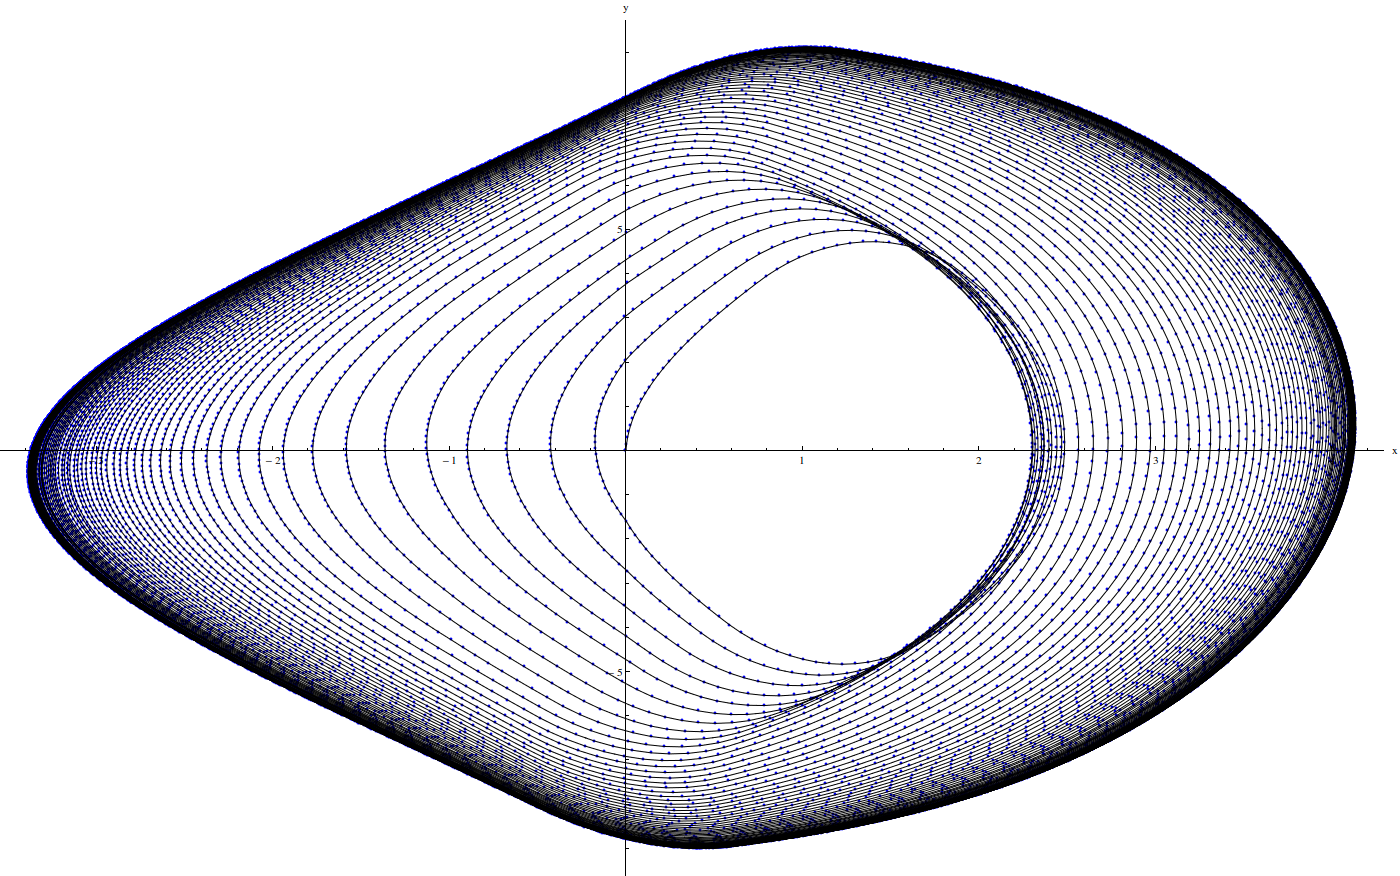
\includegraphics[width=\textwidth]{model-organisms/model-leg/Modelleg-(x)vyz-0g-force-0-00007-damping-0-joint.png}
		\end{subfigure}
	\caption[Figure of chaotic behaviors in range 2.4-3.19]{Gravity: 0g, Sensors:  Joint position \(\rightarrow\) x(t),Joint Velocity \(\rightarrow\) y(t), Output: z(t) \(\rightarrow\) Joint torque, Friction: Creature 0, Ground 0, Torque scaling curve:\(0.7~(mass_1~\cdot~mass_2)\)}

	\label{figure:z-2.4-3.19-chaotictrajectories}
\end{figure}


\begin{figure}[H]
	\centering
		\begin{subfigure}[c]{0.45\textwidth}
	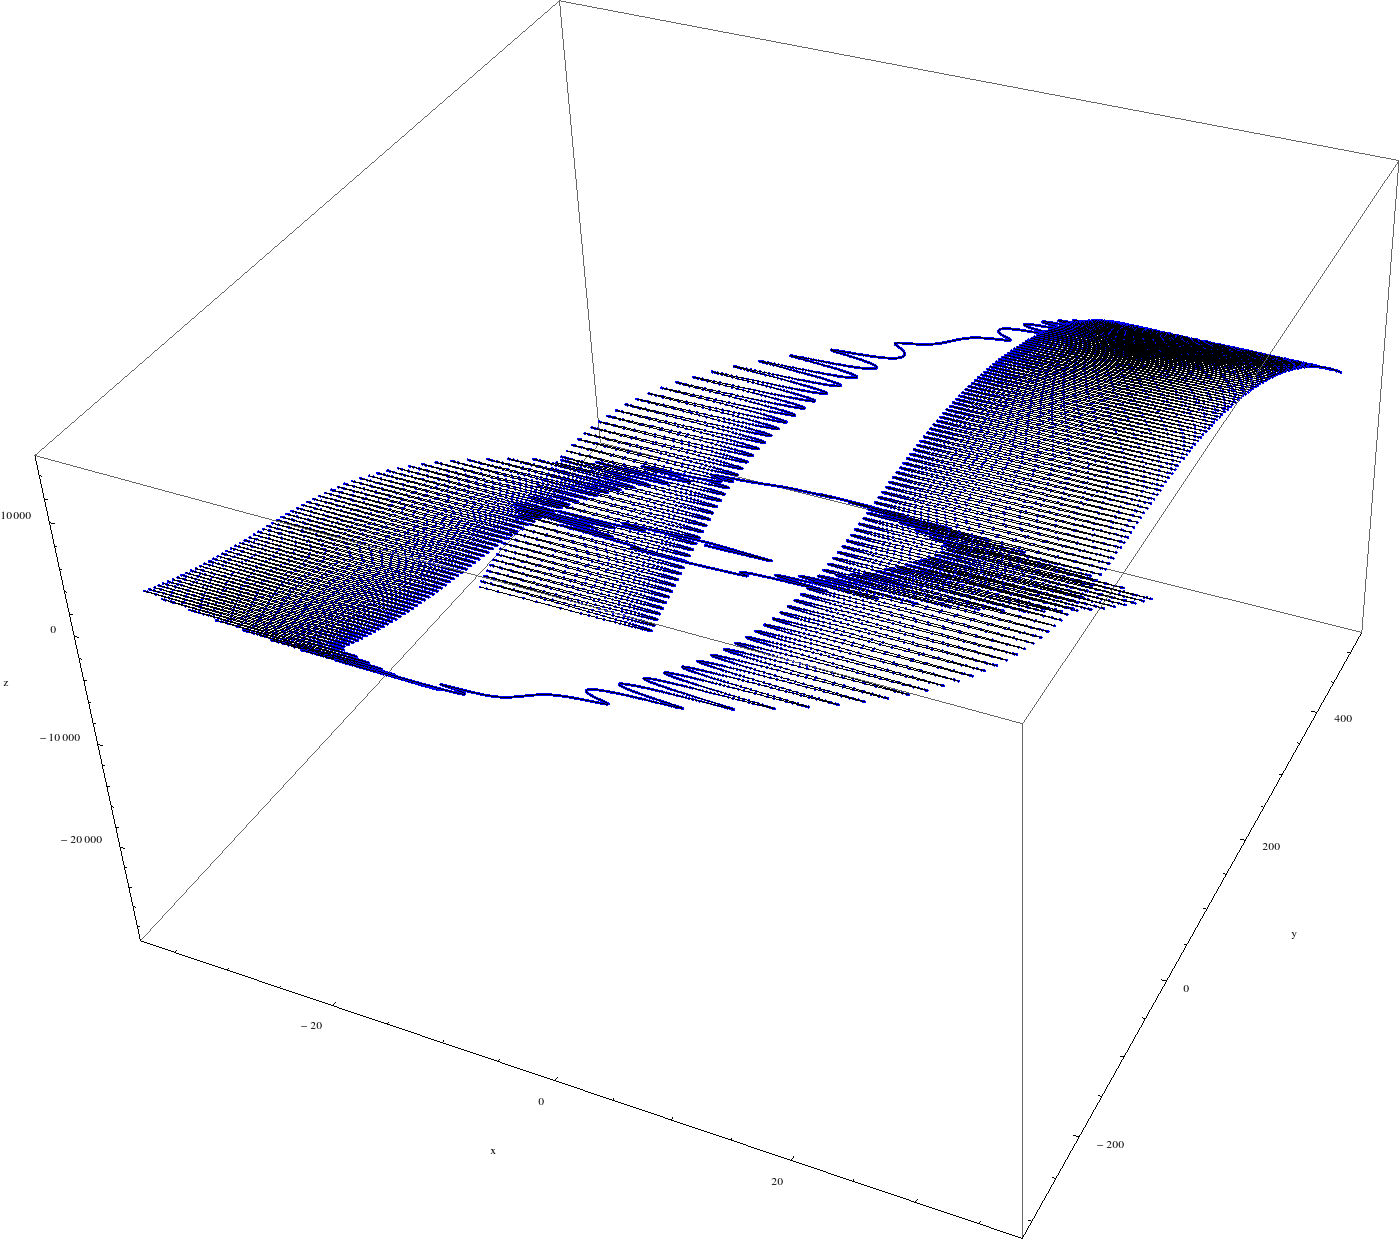
\includegraphics[width=\textwidth]{model-organisms/model-leg/Modelleg-vxpyz-0g-force-0-00007-damping-0.png}
		\end{subfigure}
	\begin{subfigure}[c]{0.45\textwidth}
	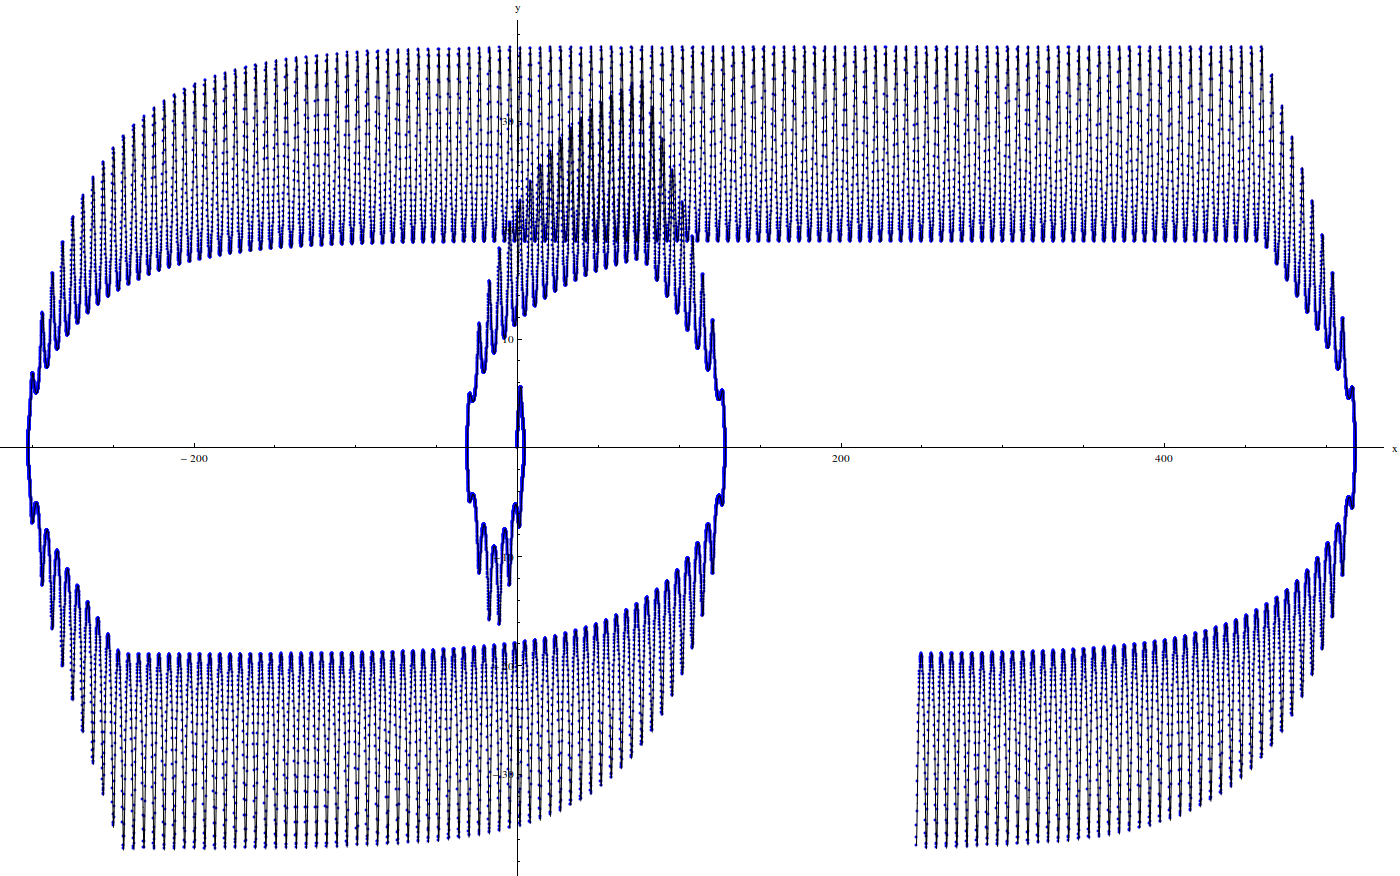
\includegraphics[width=\textwidth]{model-organisms/model-leg/Modelleg-vxpyz-0g-force-0-00007-damping-0-joint.png}
		\end{subfigure}
	\caption[Figure of chaotic behaviors in range 2.4-3.19]{Gravity: 0g, Sensors:  Joint position \(\rightarrow\) x(t),Joint Velocity \(\rightarrow\) y(t), Output: z(t) \(\rightarrow\) Joint torque, Friction: Creature 0, Ground 0, Torque scaling curve:\(0.7~(mass_1~\cdot~mass_2)\)}

	\label{figure:z-2.4-3.19-chaotictrajectories}
\end{figure}

Deciding pxvyz.  the model leg with different control torques, friction and damping coefficients was tested to observe the resulting change in controller dynamics. 

\begin{figure}[H]
	\centering
		\begin{subfigure}[c]{0.45\textwidth}
	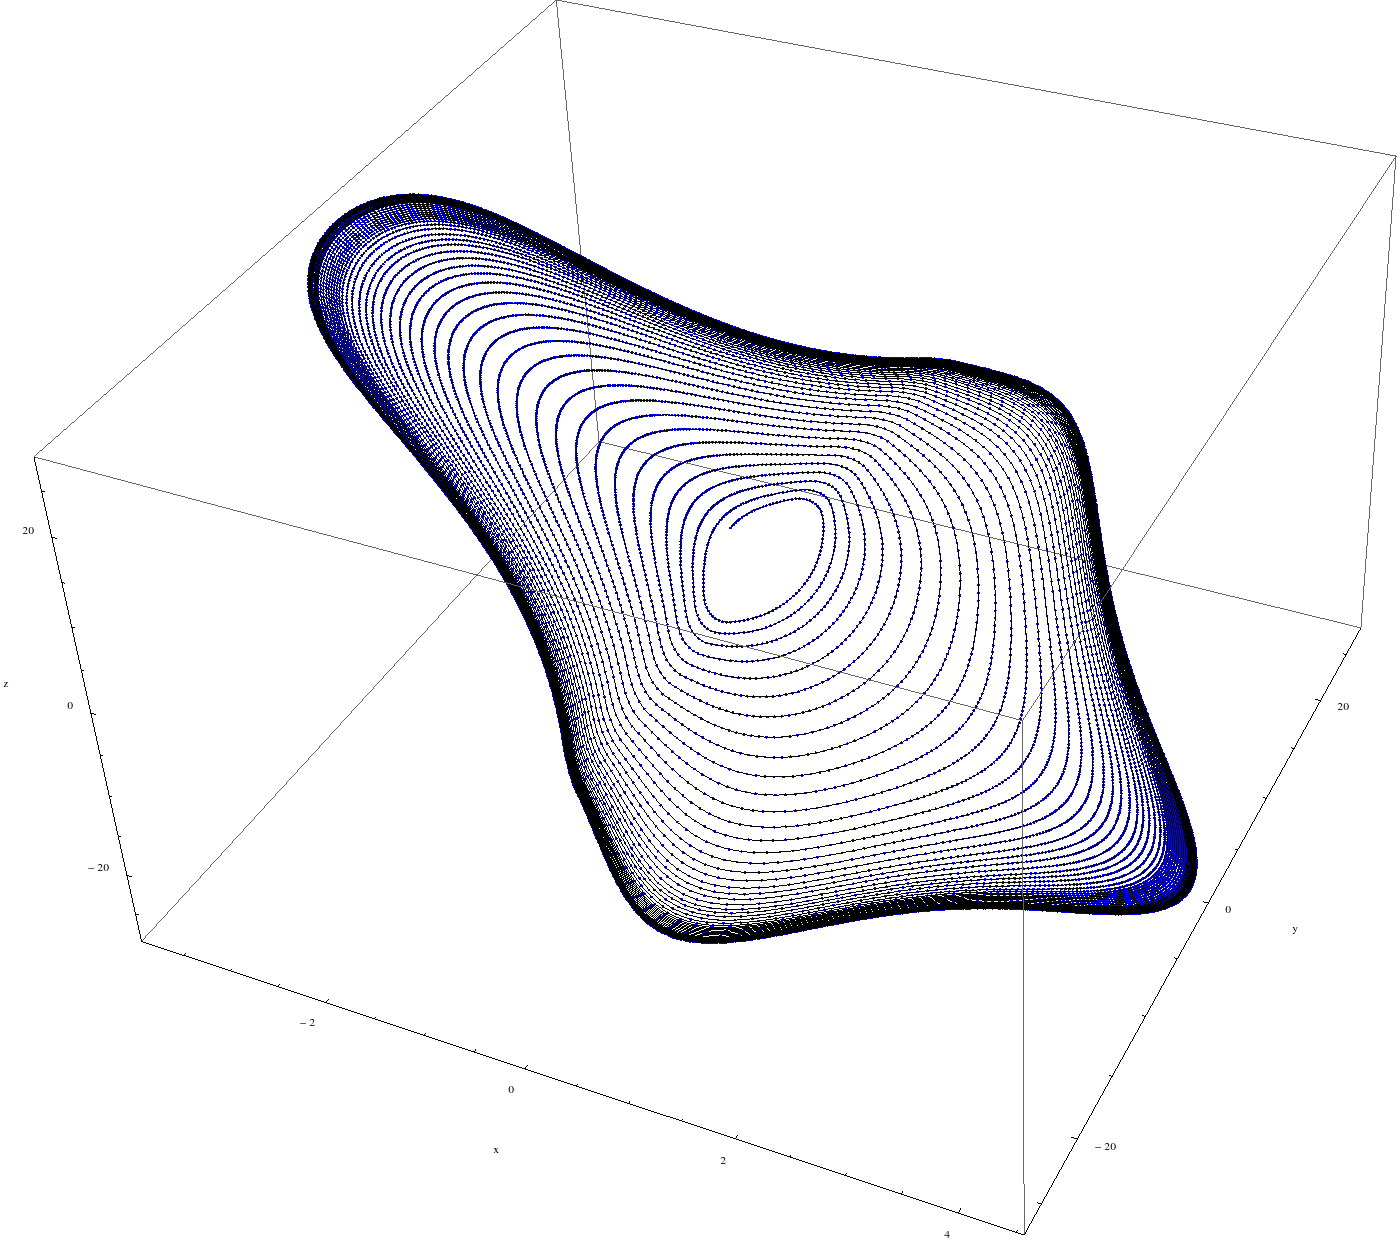
\includegraphics[width=\textwidth]{model-organisms/model-leg/Modelleg-0g-100s-friction1010-force0-7-damping0-xyz.png}
		\end{subfigure}
	\begin{subfigure}[c]{0.45\textwidth}
	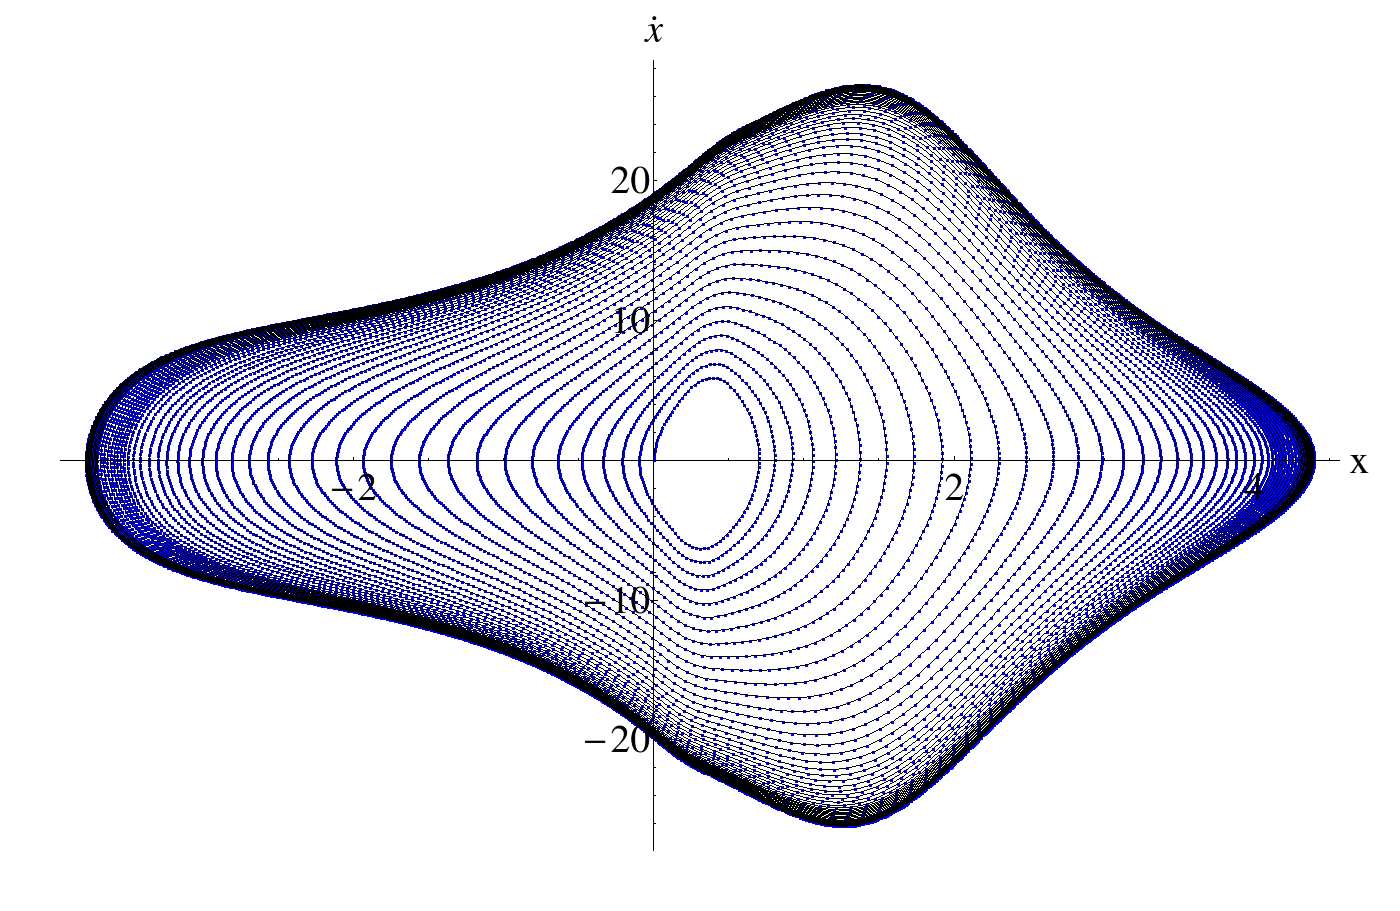
\includegraphics[width=\textwidth]{model-organisms/model-leg/Modelleg-0g-100s-friction1010-force0-7-damping0-xyz-joint.png}
		\end{subfigure}
	\caption[Figure of chaotic behaviors in range 2.4-3.19]{Gravity: 0g, Sensors:  Joint position \(\rightarrow\) x(t),Joint Velocity \(\rightarrow\) y(t), Output: z(t) \(\rightarrow\) Joint torque, Friction: Creature 0, Ground 0, Torque scaling curve:\(0.7~(mass_1~\cdot~mass_2)\)}

	\label{figure:z-2.4-3.19-chaotictrajectories}
\end{figure}

\begin{figure}[H]
	\centering
		\begin{subfigure}[c]{0.45\textwidth}
	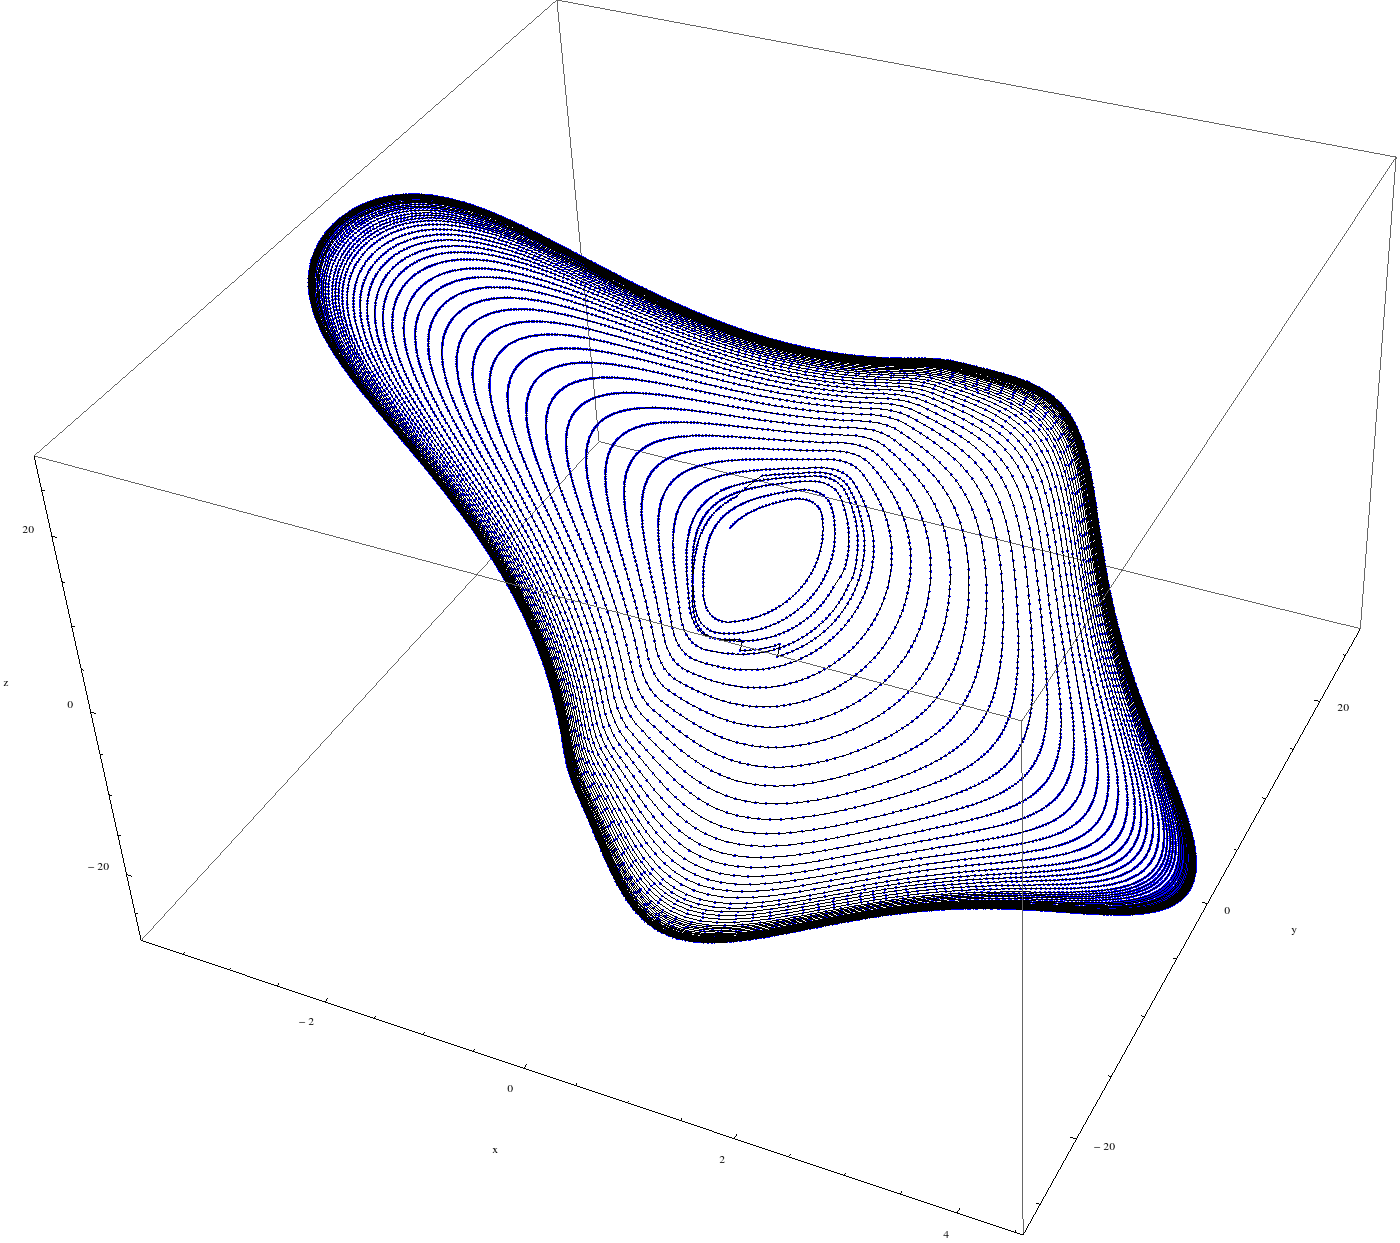
\includegraphics[width=\textwidth]{model-organisms/model-leg/Modelleg-1g-100s-friction00-force0-7-damping0-xyz.png}
		\end{subfigure}
	\begin{subfigure}[c]{0.45\textwidth}
	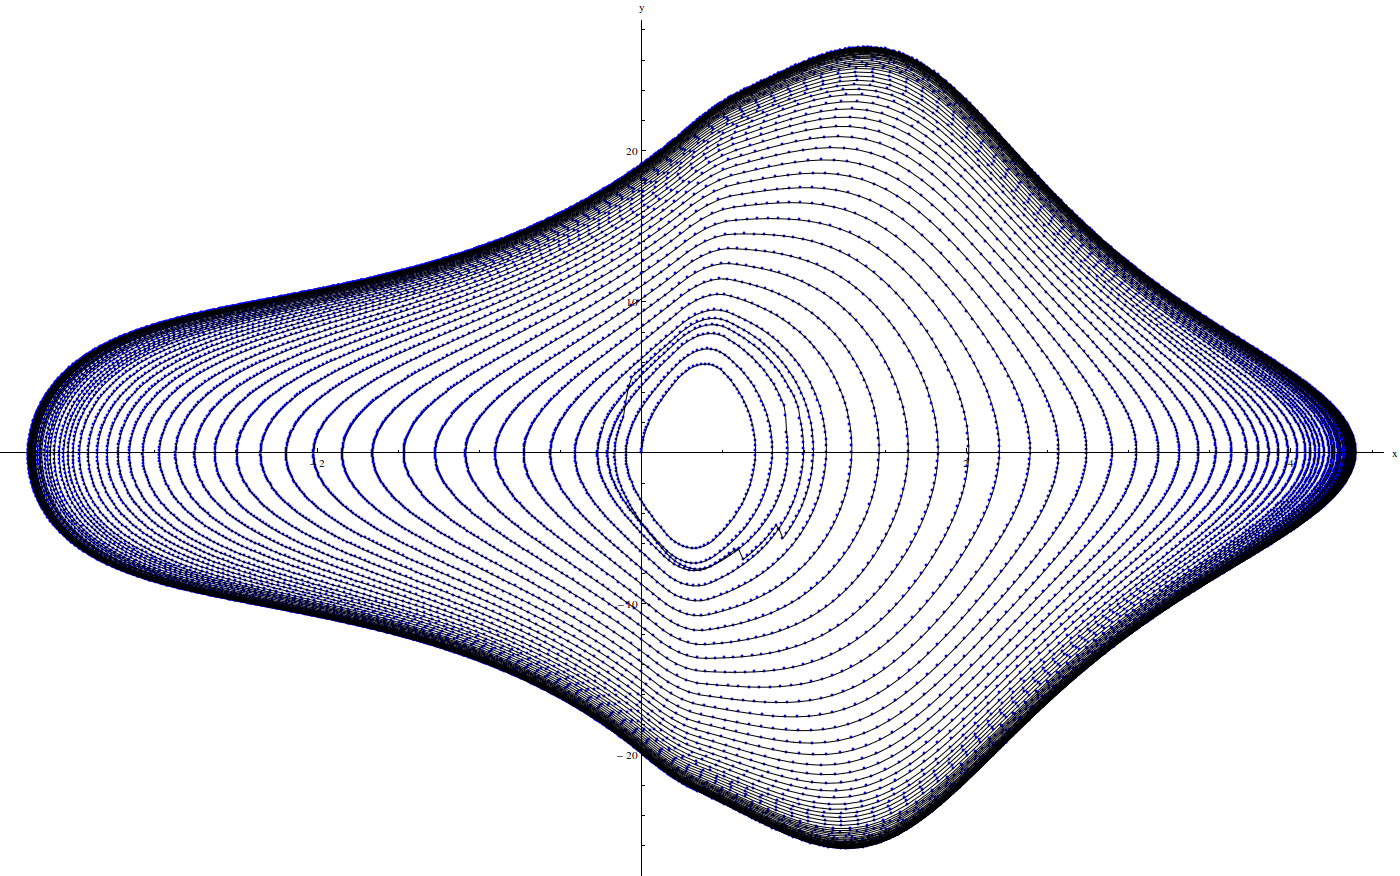
\includegraphics[width=\textwidth]{model-organisms/model-leg/Modelleg-1g-100s-friction00-force0-7-damping0-xyz-joint.png}
		\end{subfigure}
	\caption[Figure of chaotic behaviors in range 2.4-3.19]{Gravity: 0g, Sensors:  Joint position \(\rightarrow\) x(t),Joint Velocity \(\rightarrow\) y(t), Output: z(t) \(\rightarrow\) Joint torque, Friction: Creature 0, Ground 0, Torque scaling curve:\(0.7~(mass_1~\cdot~mass_2)\)}

	\label{figure:z-2.4-3.19-chaotictrajectories}
\end{figure}

\begin{figure}[H]
	\centering
		\begin{subfigure}[c]{0.45\textwidth}
	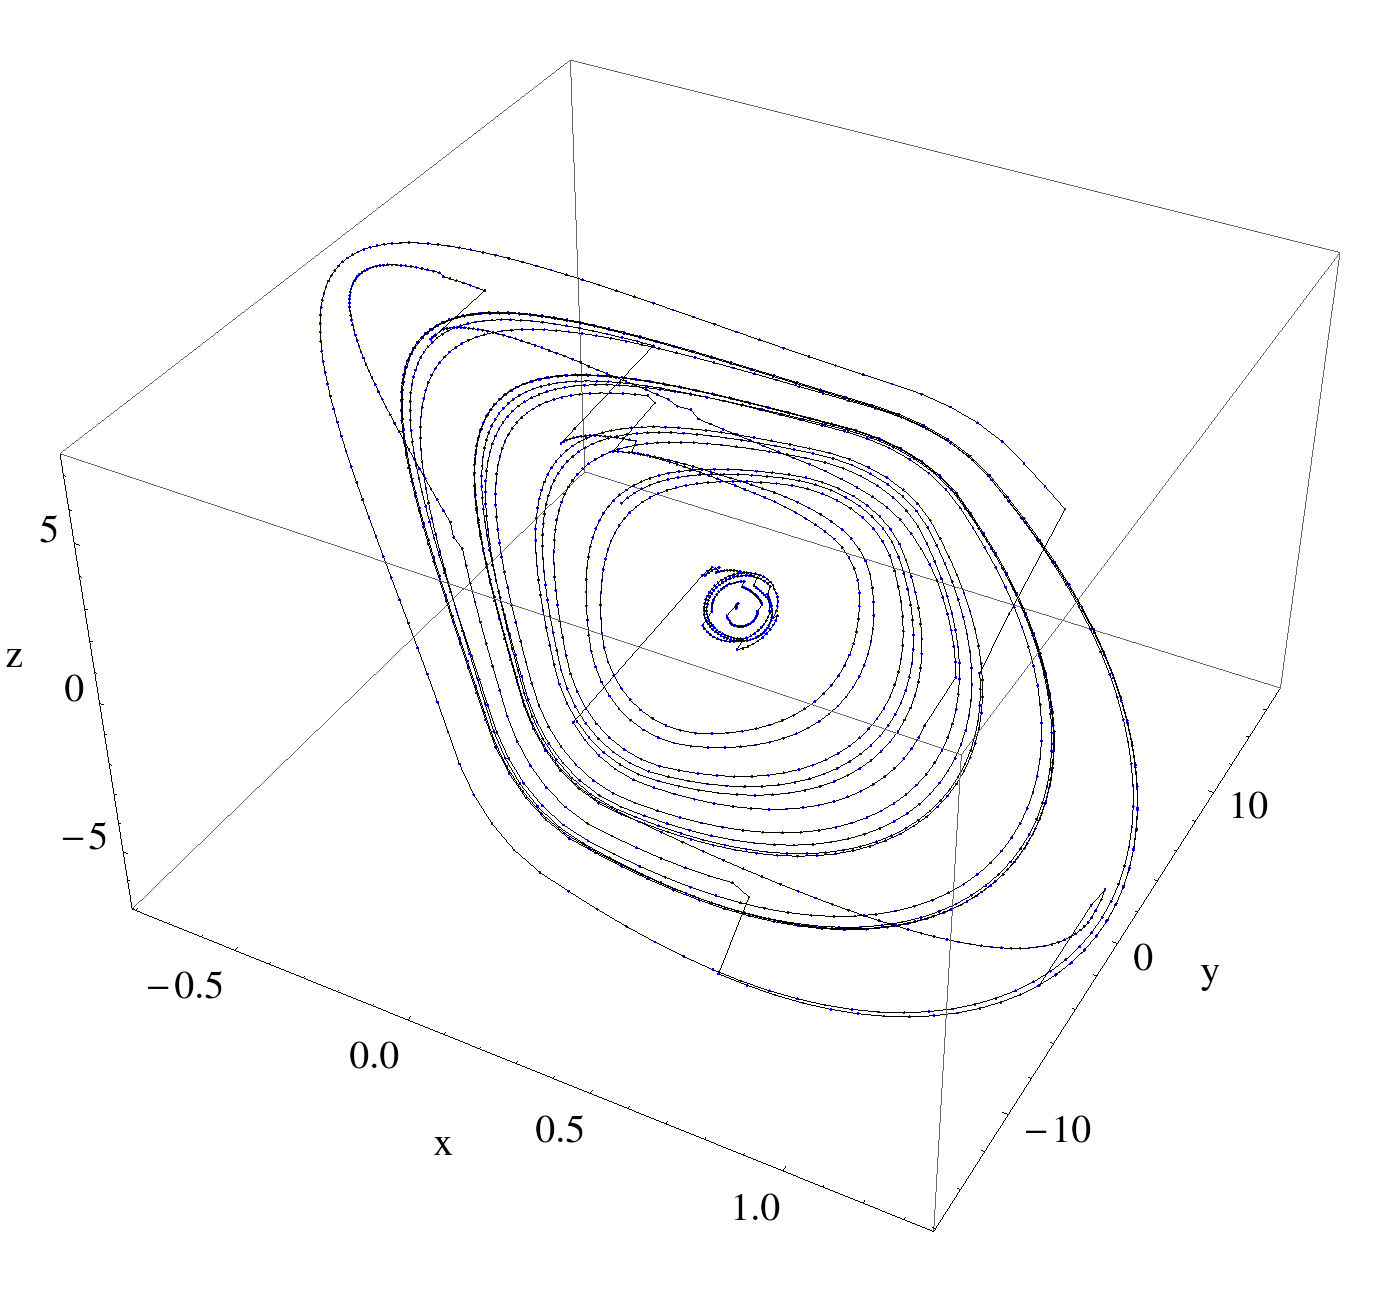
\includegraphics[width=\textwidth]{model-organisms/model-leg/Modelleg-1g-100s-friction11-force2-damping0-xyz.png}
		\end{subfigure}
	\begin{subfigure}[c]{0.45\textwidth}
	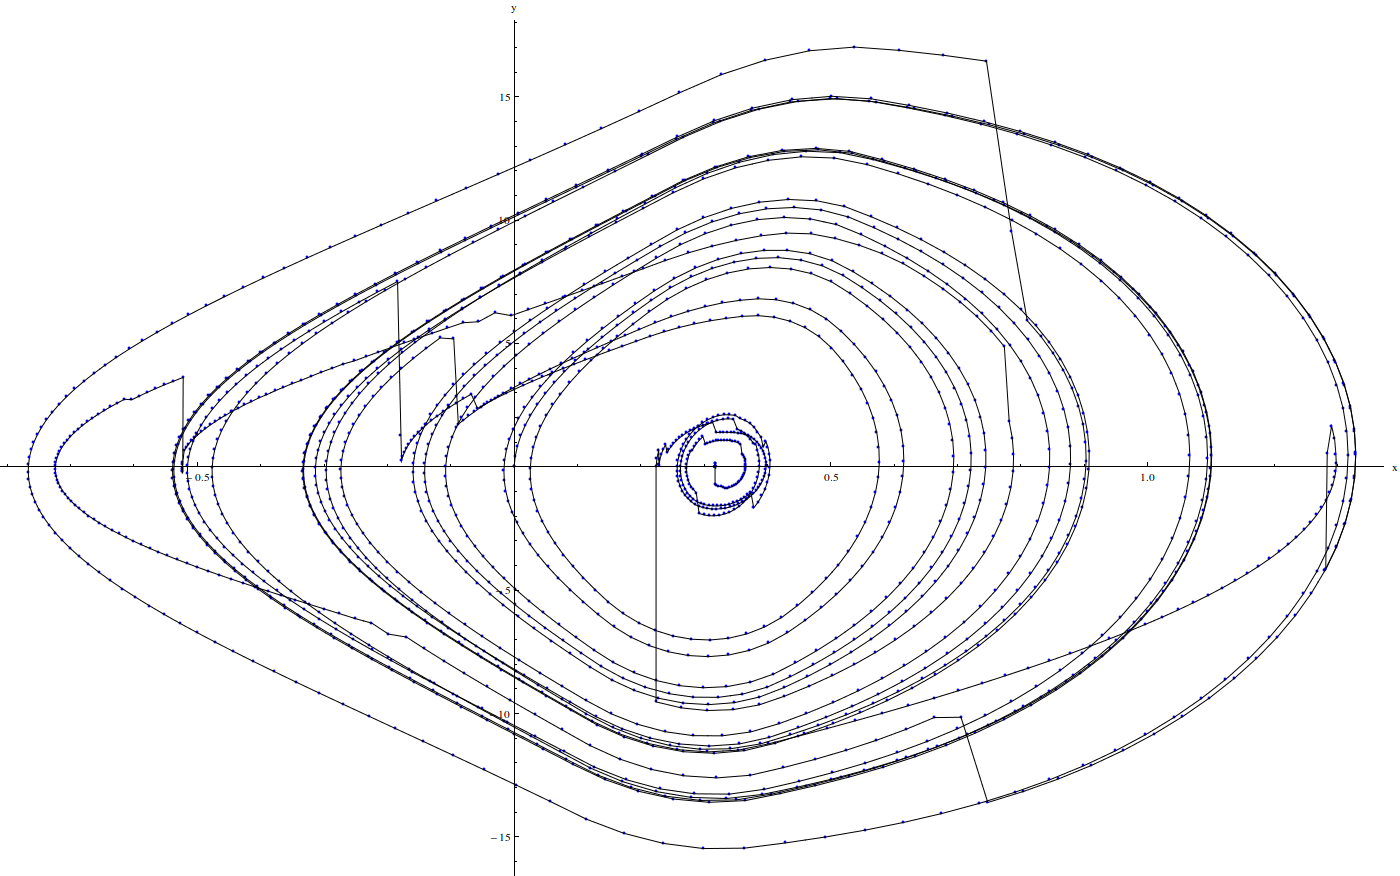
\includegraphics[width=\textwidth]{model-organisms/model-leg/Modelleg-1g-100s-friction11-force2-damping0-xyz-joint.png}
		\end{subfigure}
	\caption[Figure of chaotic behaviors in range 2.4-3.19]{Gravity: 0g, Sensors:  Joint position \(\rightarrow\) x(t),Joint Velocity \(\rightarrow\) y(t), Output: z(t) \(\rightarrow\) Joint torque, Friction: Creature 0, Ground 0, Torque scaling curve:\(0.7~(mass_1~\cdot~mass_2)\)}

	\label{figure:z-2.4-3.19-chaotictrajectories}
\end{figure}

\begin{figure}[H]
	\centering
		\begin{subfigure}[c]{0.45\textwidth}
	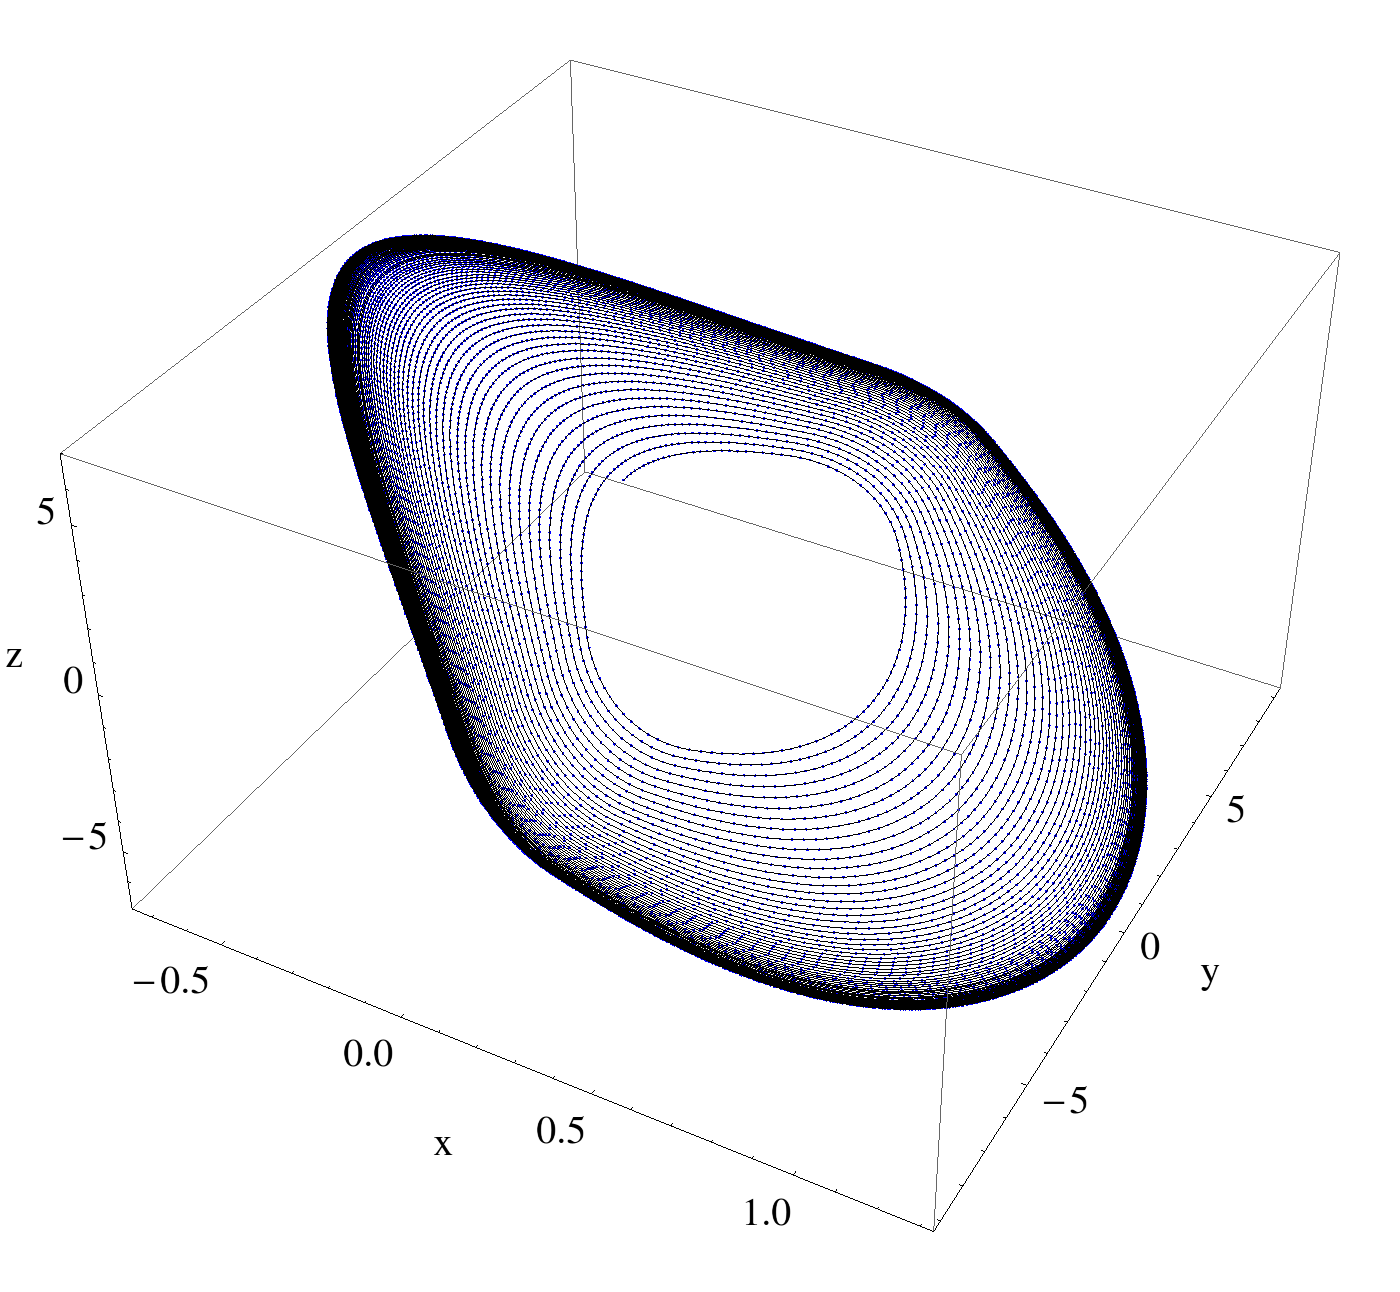
\includegraphics[width=\textwidth]{model-organisms/model-leg/Modelleg-0g-100s-friction11-force0-7-damping0-05-xyz.png}
		\end{subfigure}
	\begin{subfigure}[c]{0.45\textwidth}
	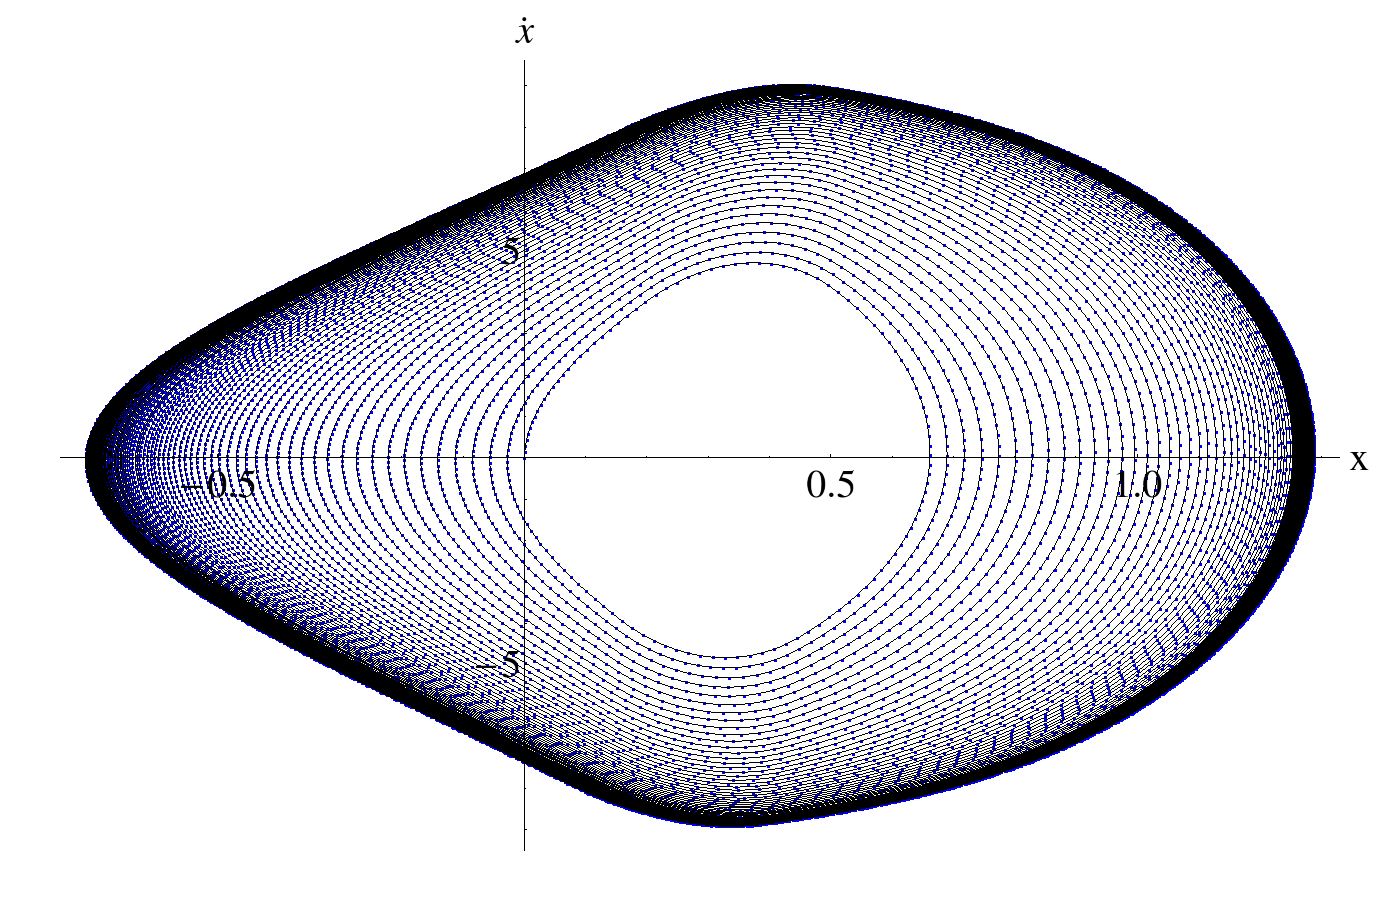
\includegraphics[width=\textwidth]{model-organisms/model-leg/Modelleg-0g-100s-friction11-force0-7-damping0-05-xyz-joint.png}
		\end{subfigure}
	\caption[Figure of chaotic behaviors in range 2.4-3.19]{Gravity: 0g, Sensors:  Joint position \(\rightarrow\) x(t),Joint Velocity \(\rightarrow\) y(t), Output: z(t) \(\rightarrow\) Joint torque, Friction: Creature 0, Ground 0, Torque scaling curve:\(0.7~(mass_1~\cdot~mass_2)\)}

	\label{figure:z-2.4-3.19-chaotictrajectories}
\end{figure}


\begin{figure}[H]
	\centering
		\begin{subfigure}[c]{0.45\textwidth}
	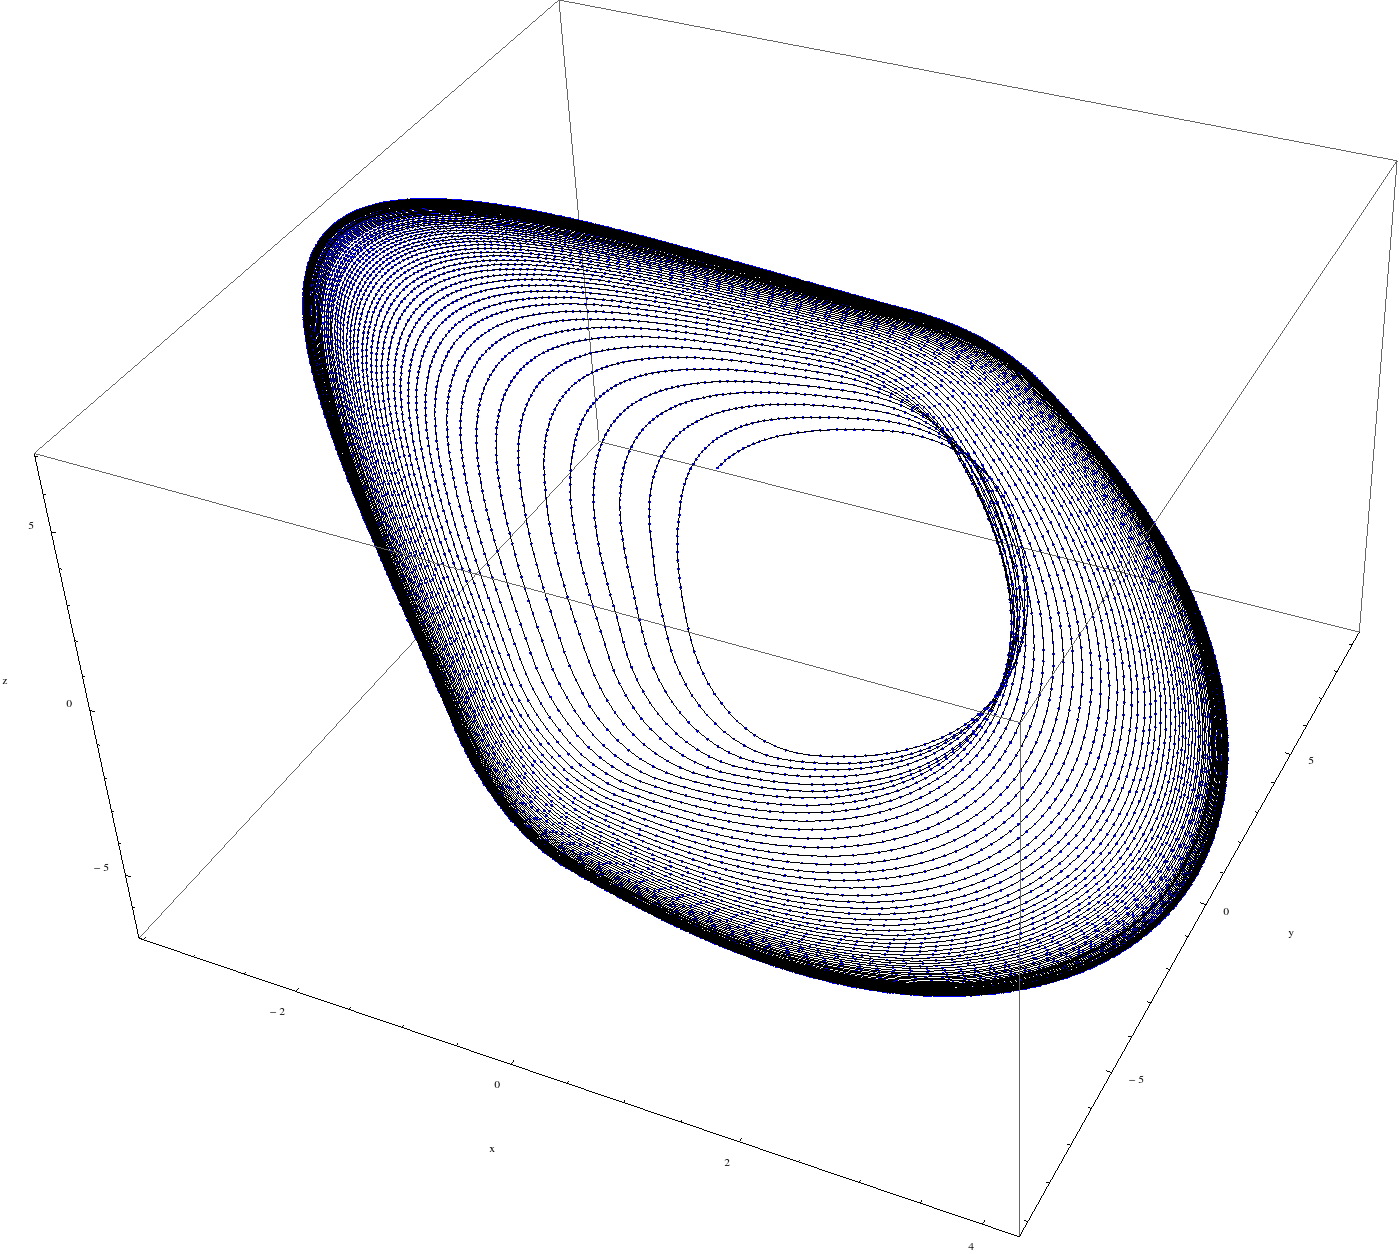
\includegraphics[width=\textwidth]{model-organisms/model-leg/Modelleg-0g-100s-friction11-force0-7-damping0-05-(x)yz.png}
		\end{subfigure}
	\begin{subfigure}[c]{0.45\textwidth}
	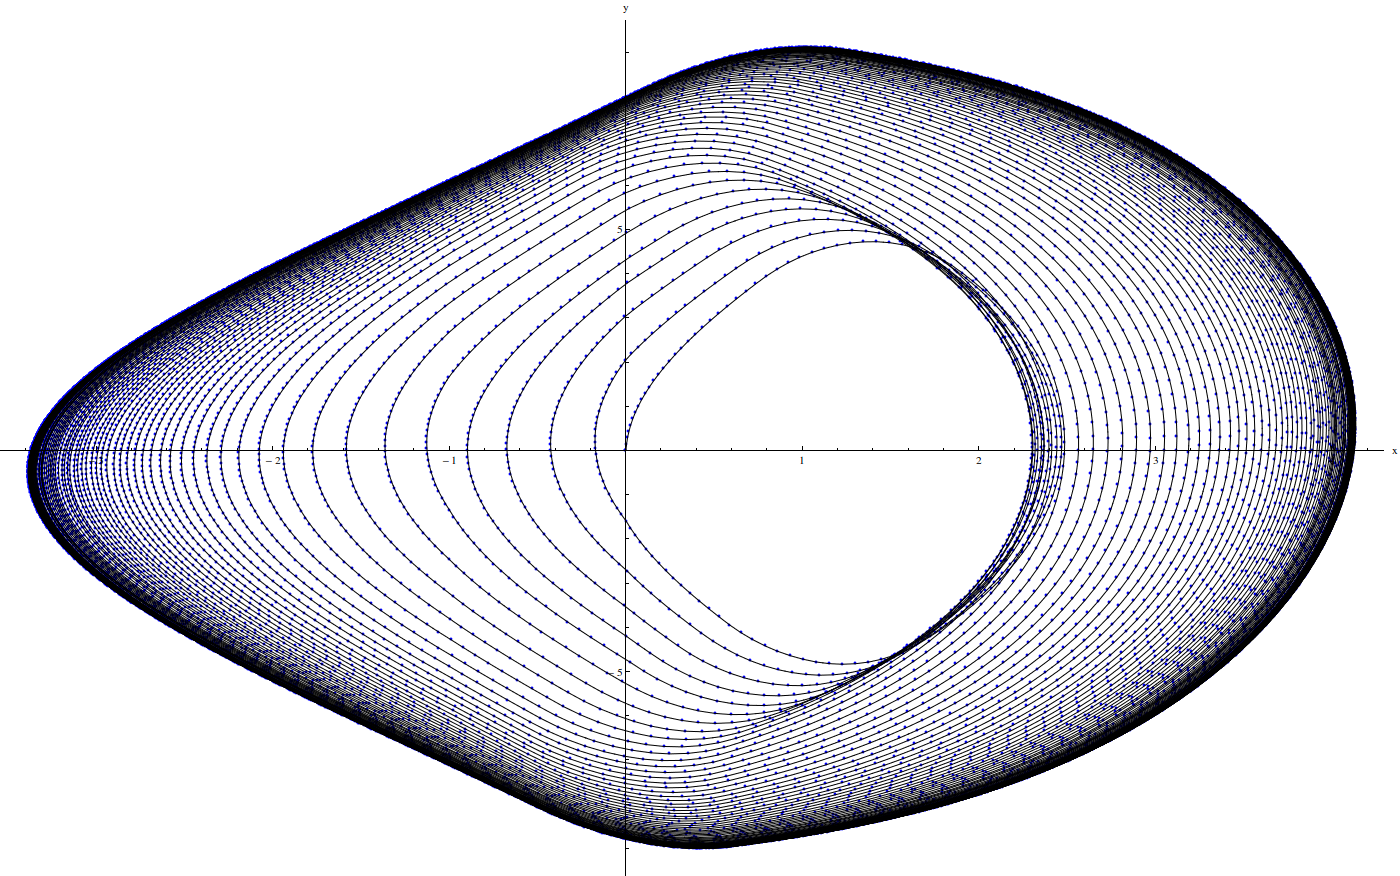
\includegraphics[width=\textwidth]{model-organisms/model-leg/Modelleg-0g-100s-friction11-force0-7-damping0-05-(x)yz-joint.png}
		\end{subfigure}
	\caption[Figure of chaotic behaviors in range 2.4-3.19]{Gravity: 0g, Sensors:  Joint position \(\rightarrow\) x(t),Joint Velocity \(\rightarrow\) y(t), Output: z(t) \(\rightarrow\) Joint torque, Friction: Creature 0, Ground 0, Torque scaling curve:\(0.7~(mass_1~\cdot~mass_2)\)}

	\label{figure:z-2.4-3.19-chaotictrajectories}
\end{figure}

\begin{figure}[H]
	\centering
		\begin{subfigure}[c]{0.45\textwidth}
	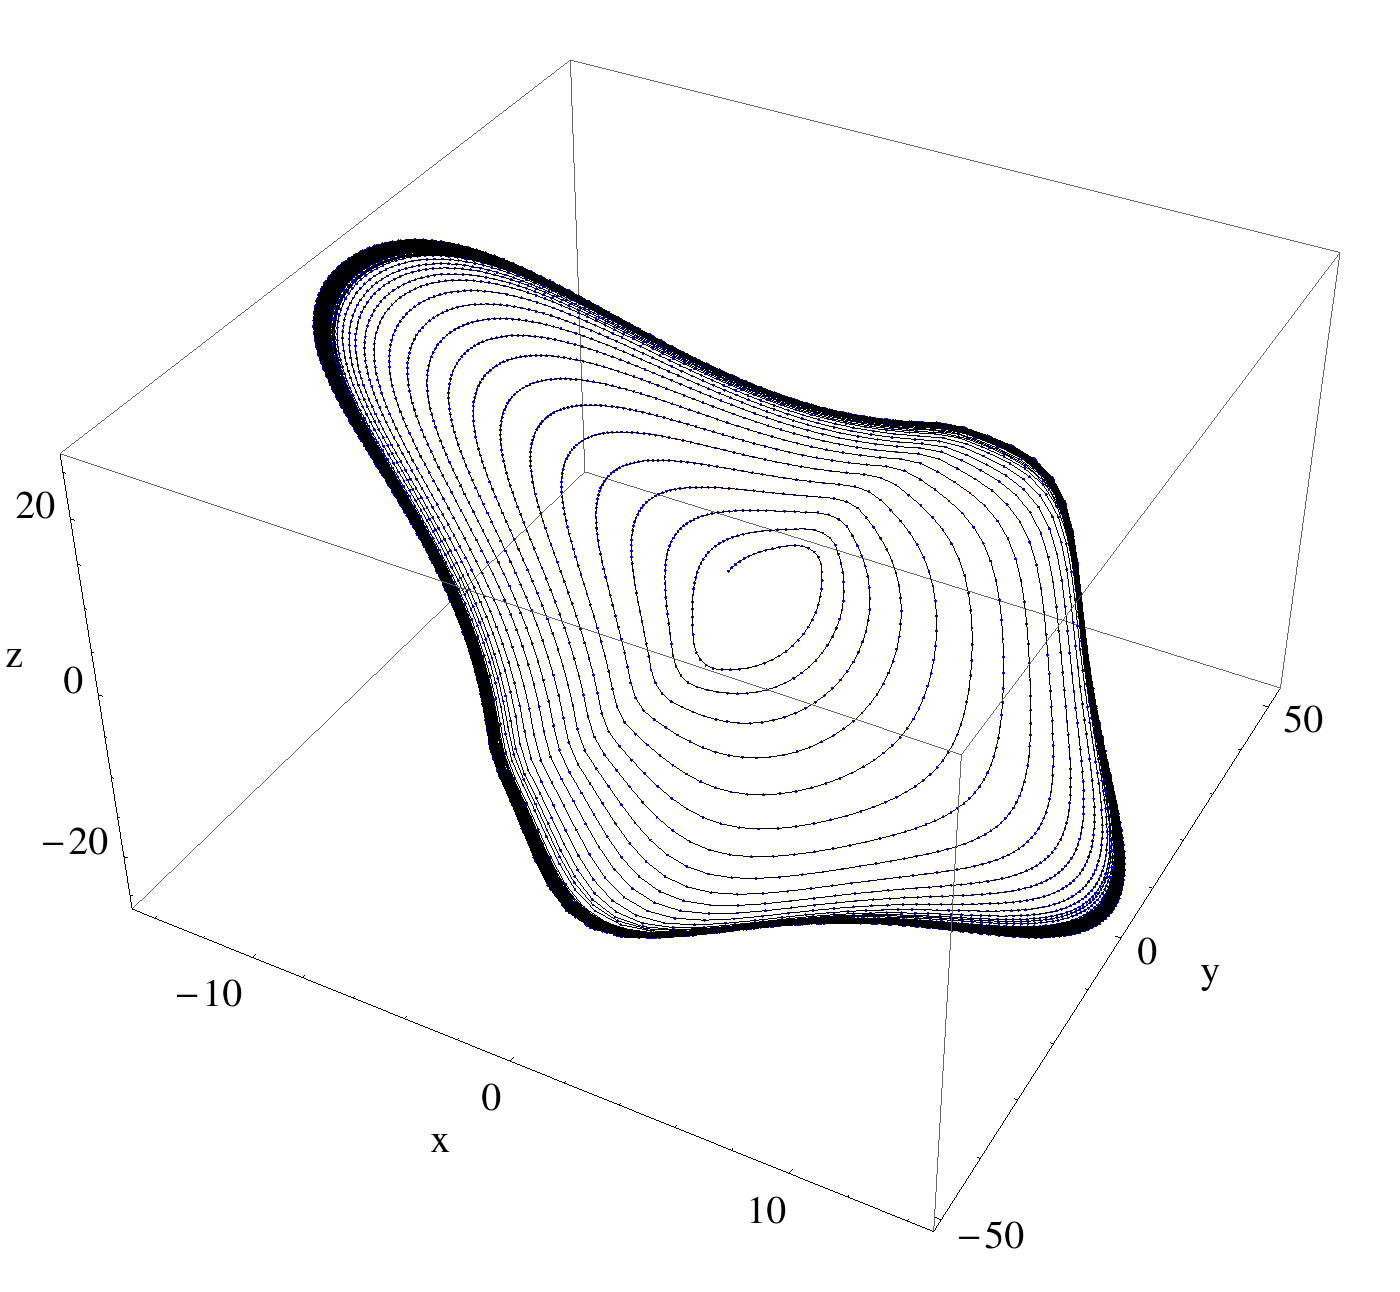
\includegraphics[width=\textwidth]{model-organisms/model-leg/Modelleg-0g-100s-friction11-force4-damping0-05-(x)yz.png}
		\end{subfigure}
	\begin{subfigure}[c]{0.45\textwidth}
	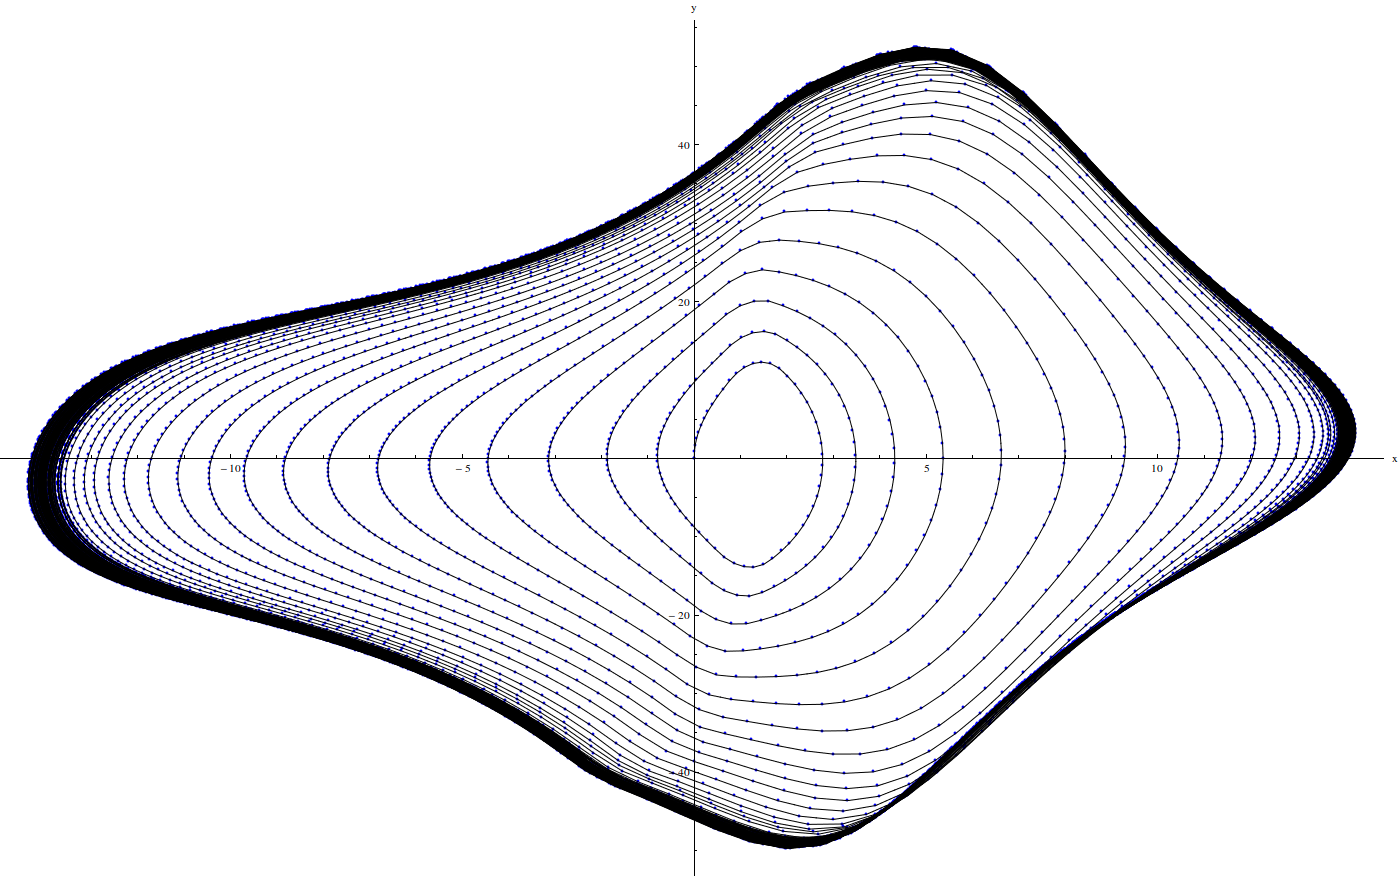
\includegraphics[width=\textwidth]{model-organisms/model-leg/Modelleg-0g-100s-friction11-force4-damping0-05-(x)yz-joint.png}
		\end{subfigure}
	\caption[Figure of chaotic behaviors in range 2.4-3.19]{Gravity: 0g, Sensors:  Joint position \(\rightarrow\) x(t),Joint Velocity \(\rightarrow\) y(t), Output: z(t) \(\rightarrow\) Joint torque, Friction: Creature 0, Ground 0, Torque scaling curve:\(0.7~(mass_1~\cdot~mass_2)\)}

	\label{figure:z-2.4-3.19-chaotictrajectories}
\end{figure}

\begin{figure}[H]
	\centering
		\begin{subfigure}[c]{0.45\textwidth}
	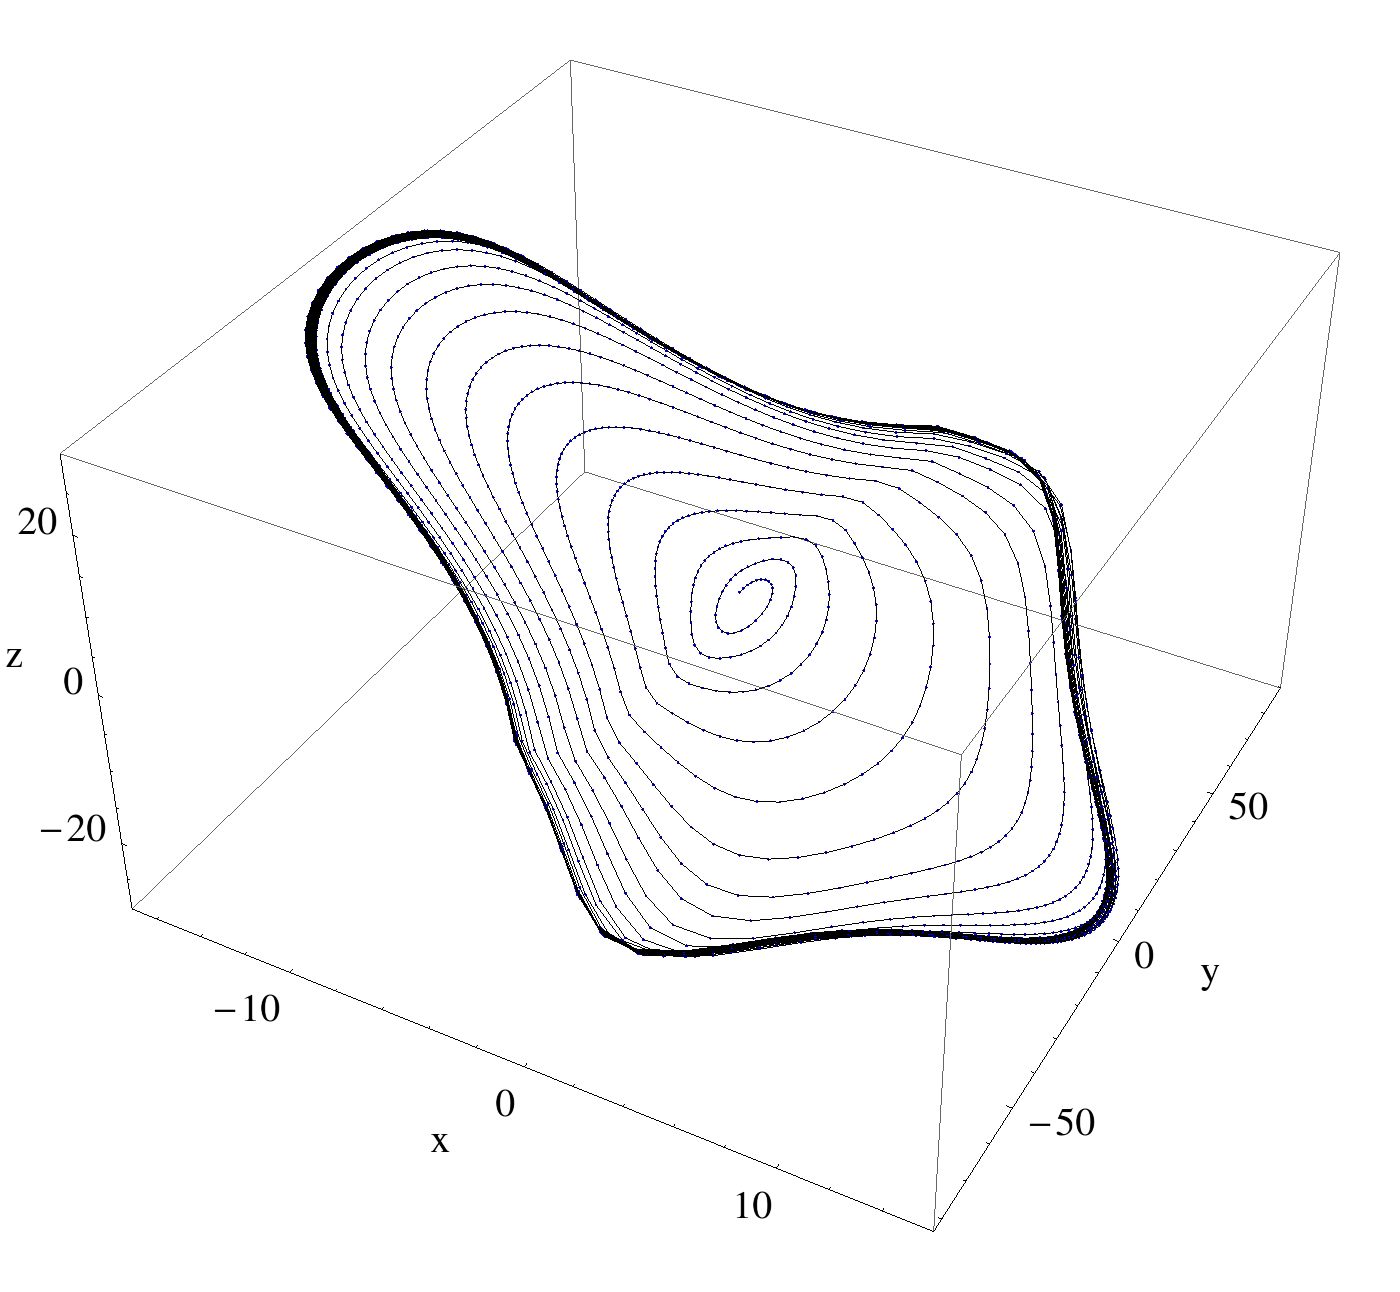
\includegraphics[width=\textwidth]{model-organisms/model-leg/Modelleg-0g-100s-friction00-force10-damping0-05-(x)yz(0-7).png}
		\end{subfigure}
	\begin{subfigure}[c]{0.45\textwidth}
	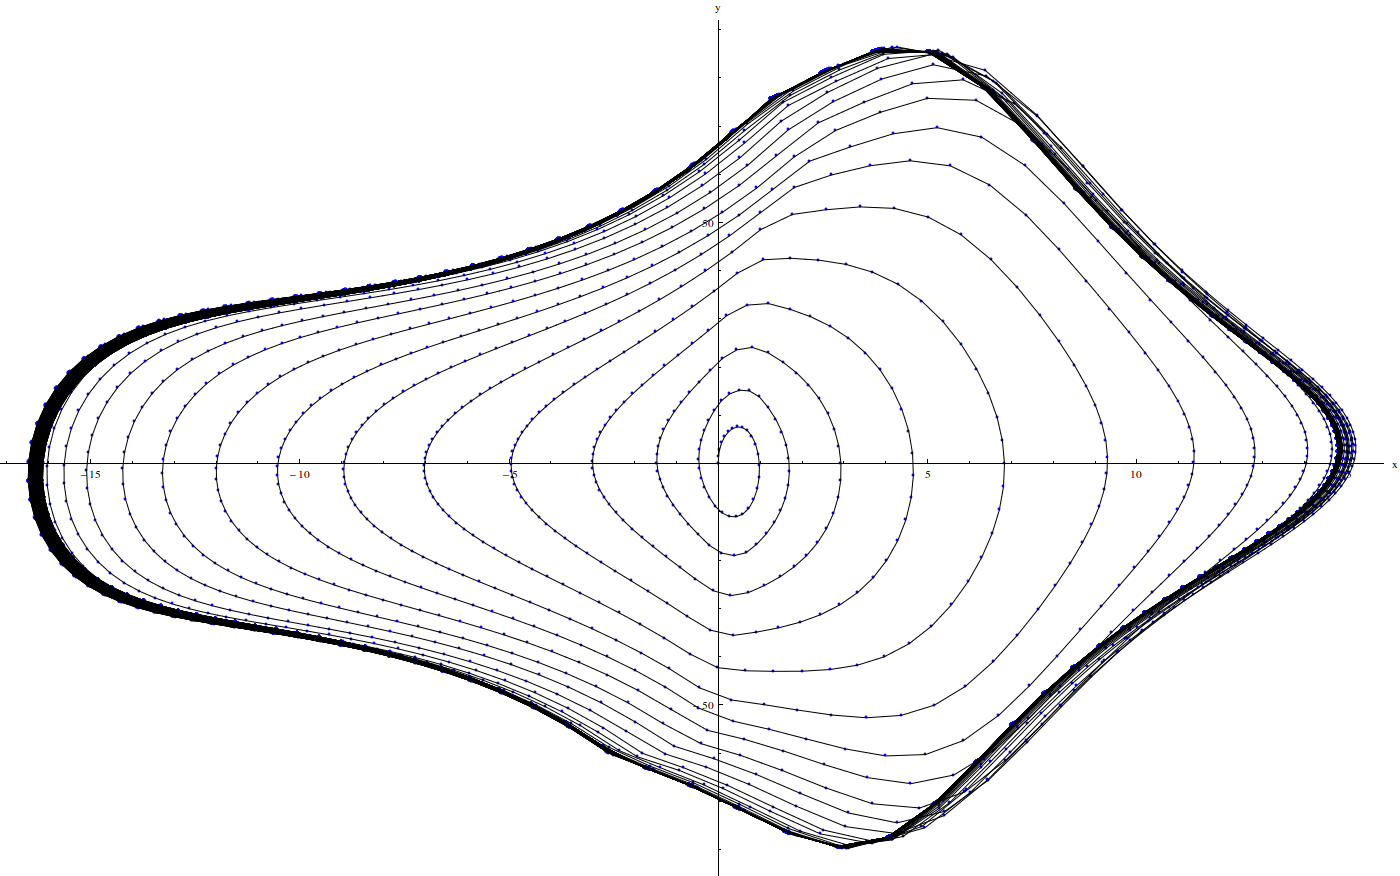
\includegraphics[width=\textwidth]{model-organisms/model-leg/Modelleg-0g-100s-friction00-force10-damping0-05-(x)yz(0-7)-joint.png}
		\end{subfigure}
	\caption[Figure of chaotic behaviors in range 2.4-3.19]{Gravity: 0g, Sensors:  Joint position \(\rightarrow\) x(t),Joint Velocity \(\rightarrow\) y(t), Output: z(t) \(\rightarrow\) Joint torque, Friction: Creature 0, Ground 0, Torque scaling curve:\(0.7~(mass_1~\cdot~mass_2)\)}

	\label{figure:z-2.4-3.19-chaotictrajectories}
\end{figure}

\begin{figure}[H]
	\centering
		\begin{subfigure}[c]{0.45\textwidth}
	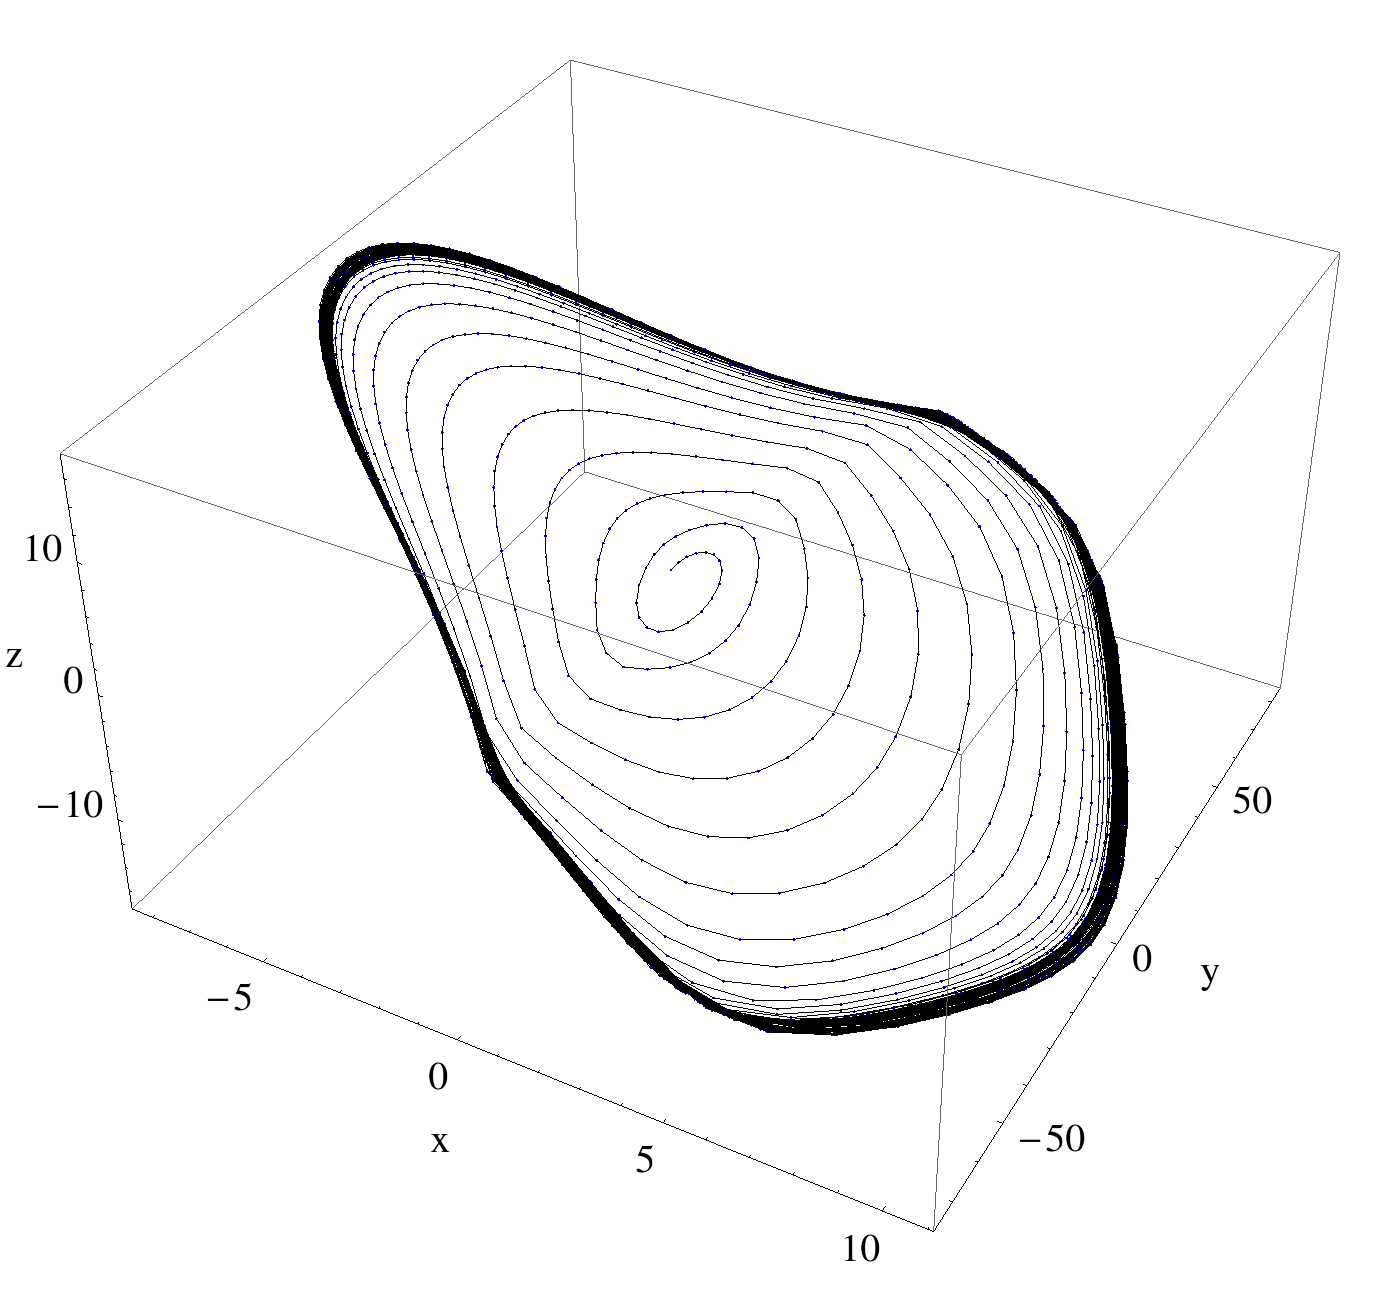
\includegraphics[width=\textwidth]{model-organisms/model-leg/Modelleg-0g-100s-friction00-force20-damping5-(x)yz(0-7).png}
		\end{subfigure}
	\begin{subfigure}[c]{0.45\textwidth}
	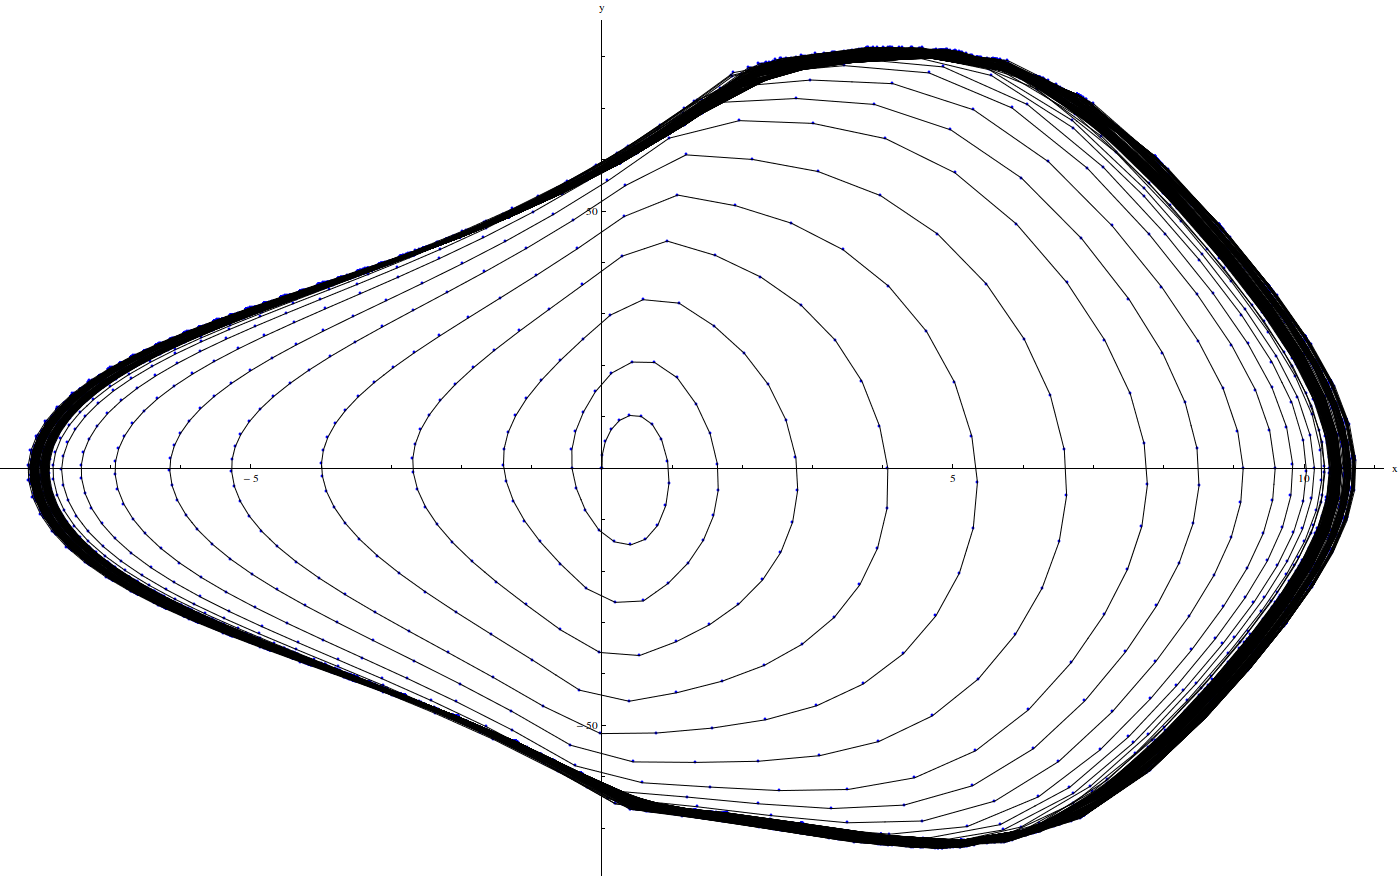
\includegraphics[width=\textwidth]{model-organisms/model-leg/Modelleg-0g-100s-friction00-force20-damping5-(x)yz(0-7)-joint.png}
		\end{subfigure}
	\caption[Figure of chaotic behaviors in range 2.4-3.19]{Gravity: 0g, Sensors:  Joint position \(\rightarrow\) x(t),Joint Velocity \(\rightarrow\) y(t), Output: z(t) \(\rightarrow\) Joint torque, Friction: Creature 0, Ground 0, Torque scaling curve:\(0.7~(mass_1~\cdot~mass_2)\)}

	\label{figure:z-2.4-3.19-chaotictrajectories}
\end{figure}

\begin{minipage}{\textwidth}
\begin{minipage}{0.5\textwidth}

   \begin{figure}[H]
	\centering
	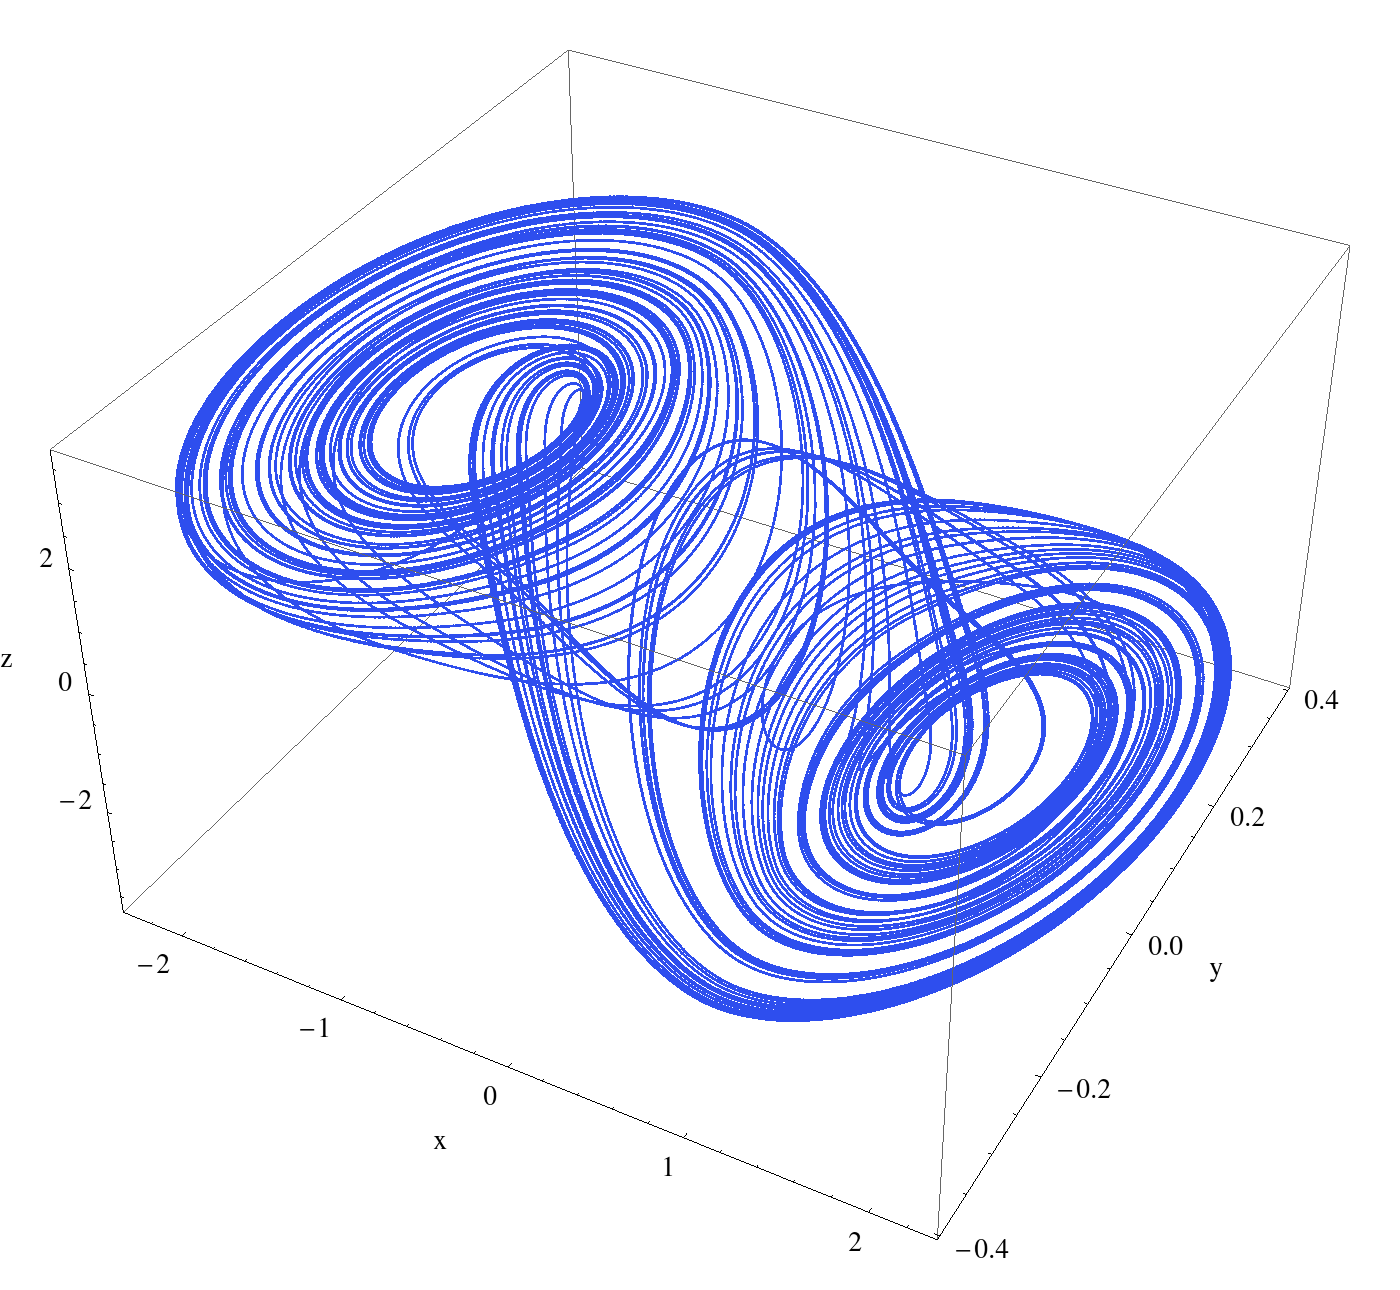
\includegraphics[width=\textwidth]{chua-circuit/Limited-chua-circuit-z-softness-0-13-3.png}
	\caption[Figure of chaotic behaviors in range 2.4-3.19]{Figure of chaotic behaviors in range 2.4-3.19. The limit values of the shown figures are \(3\), \(2.8\), \(2.6\) and \(2.4\).}
	\label{figure:z-2.4-3.19-chaotictrajectories}
	\end{figure}
	
\end{minipage}\hfill
\begin{minipage}{0.5\textwidth}
	\scriptsize
   \begin{itemize}
		\item Gravity: 0g
		\item Sensors: 
		\begin{itemize}
			\item Joint position \(\rightarrow\) x(t)
			\item Joint Velocity \(\rightarrow\) y(t)
		\end{itemize}
		\item Output: z(t) \(\rightarrow\) Joint torque
		\item Friction: Creature 10, Ground 10
		\item \mbox{Torque scaling curve:} \(0.7~(mass_1~\cdot~mass_2)\)
	\end{itemize}
	\normalsize
	
\end{minipage}%
\end{minipage}

\todo[inline]{Finish section on model leg experiments.}

\subsubsection{Evolving creatures with direct limiter control}

\lipsum{1}

\todo[inline]{Write about evolving creatures with direct limiter control}

\end{document}